%\documentclass[11pt,twoside]{article}
\documentclass[11pt,twoside,pdftex]{article}

\usepackage{color}
\definecolor{darkgray}{gray}{0.20}

\usepackage{geometry}
\geometry{verbose,a4paper,tmargin=2.54cm,bmargin=2.54cm,inner=3.17cm,outer=2.54cm}

\usepackage{hyperref}  %EXAMPLE: \href{http://www.niwa.co.nz}{NIWA}
\hypersetup{
  breaklinks=true,      % allow line breaks in URLs
  colorlinks=true,      % use colour to define links
  linkcolor=black,      % colour of internal links
  citecolor=black,      % colour of links to bibliography
  filecolor=black,      % colour of file links
  urlcolor=darkgray     % colour of external links
}

%Graphics (no postscript files.. just use jpeg, png, etc)
\usepackage[dvips]{graphicx}
\usepackage{pslatex}

% Referencing
\usepackage{natbib}
\bibliographystyle{plainnat}
\renewcommand{\bibsection}{%
  \section{References}}
  \setcitestyle{round,aysep={},yysep={;}%
}

%Page style
\usepackage{fancyhdr}
\pagestyle{fancy}
\fancyhead{}
\fancyfoot{}
\headheight 25pt 
\renewcommand{\headrulewidth}{0pt}
\renewcommand{\footrulewidth}{0pt}
\setlength{\parskip}{\medskipamount}
\setlength{\parindent}{0pt}

%Verbatim enviroment
\usepackage{fancyvrb}

% New commands to define macros and other aids to text and layout
\newcommand{\config}{`input configuration file'}
\newcommand{\command}[2] {\texttt{@#1\ #2}}
\newcommand{\subcommand}[2] {\texttt{#1 \ #2}}
\newcommand{\commandlabel}[1]{\texttt{#1}}
\newcommand{\commentline}{\#}
\newcommand{\commentstart}{\{}
\newcommand{\commentend}{\}}
\newcommand{\Rzero}{\emph{R}$_0$}
\newcommand{\Bzero}{\emph{B}$_0$}

%New commands to template syntax definitions
%Define null command
\newcommand{\Null}[1]{}
% Define a command without a label
\newcommand{\defCom}[2]{
 \begin{tabular}{l l}
  \texttt{\textbf{@#1}}\ & {#2} 
 \end{tabular}
}
% Define a command with a label
\newcommand{\defComLab}[2]{
 \begin{tabular}{l l}
  \texttt{\textbf{@#1}\ \emph{label}} & {#2}
 \end{tabular}
}
% Define a command with an argument
\newcommand{\defComArg}[3]{
 \begin{tabular}{l l}
  \texttt{\textbf{@#1}\ #2} & {#3}
 \end{tabular}
}
% Define a Command argument
\newcommand{\defArg}[2]{
 \begin{tabular}{l l}
  \texttt{#1}\ & #2
 \end{tabular} \\*
}
% Define a subcommand
\newcommand{\defSub}[2]{
 \begin{tabular}{l l}
  \texttt{#1}\ & #2
 \end{tabular} \\*
}
% Define subcommand types, confditions, etc.
\newcommand{\defType}[1]{\hspace*{0.5cm}Type: {#1} \\*}
\newcommand{\defDefault}[1]{\hspace*{0.5cm}Default: {#1} \\*}
\newcommand{\defCondition}[1]{\hspace*{0.5cm}Conditions: {#1} \\*}
\newcommand{\defEffect}[1]{\hspace*{0.5cm}Effect: {#1} \\*}
\newcommand{\defNote}[1]{\hspace*{0.5cm}Note: {#1} \\*}
\newcommand{\defExample}[1]{\hspace*{0.5cm}Example: {#1} \\*}

%Begin the document
\begin{document}

% Input SVN version definitions
%============================================================================
% svn_version : A command line utility to extract source control revision
%               number, date, and time.
% Author      : S.Rasmussen / A.Dunn
% Copyright   : Copyright NIWA (c)2008 - www.niwa.co.nz
%============================================================================

% Warning: This file is an atomatically generated file describing the source
% control revision number, date, and time using svn_version.

% Call: svn_version --format tex --recursive --quiet --suffix Doc 
% Current working directory: C:\Projects\General\SPM\doc\manual

\newcommand{\SourceControlRevisionDoc}{3012}
\newcommand{\SourceControlDateDoc}{2009-02-27}
\newcommand{\SourceControlYearDoc}{2009}
\newcommand{\SourceControlMonthDoc}{February}
\newcommand{\SourceControlTimeDoc}{04:09:22}
\newcommand{\SourceControlVersionDoc}{2009-02-27-04:09:22 UTC (rev. 3012)}


\newcommand{\DocYear}{\SourceControlYearDoc}
\newcommand{\DocMonth}{\SourceControlMonthDoc}
\newcommand{\DocDate}{\SourceControlMonthDoc\ \SourceControlYearDoc}
\newcommand{\DocVer}{\SourceControlDateDoc}

1.00-2009-05-18 (rev. 3364)

\newcommand{\VER}{0.2-\SourceControlDateSPM}

%New commands to automate document dates, manual titles, etc.
\newcommand{\SPM}{\texttt{SPM}}
\newcommand{\SPMName}{Spatial Population Model}
\newcommand{\authors}{\href{mailto:"Alistair Dunn"<a.dunn@niwa.co.nz>?subject=SPM:}{authors}}
\newcommand{\Organisation}{National Institute of Water \& Atmospheric Research Ltd.}
\newcommand{\ManualRef}{Dunn, A.; Rasmussen, S. (\DocYear) \SPMName\ User Manual (\SPM\ v\VER). \Organisation\ \emph{Unpublished report}.} 
\title{\SPMName\ User Manual \\(\SPM\ v\VER)}
\author{Alistair Dunn, Scott Rasmussen}
\date{\DocDate}

% Title page

\maketitle 
\thispagestyle{empty}
~\vfill
\begin{center}
\SPMName\ User Manual (modified: \DocVer) \\
for use with \SPM\ v\VER-\SourceControlTimeSPM\ UTC.
\end{center}

% Citation page
\cleardoublepage{}
\fancyfoot[C]{\thepage}
\pagenumbering{roman}
~\vfill
\begin{center}
{Citation:\\ \ManualRef}
\end{center}

% Table of contents
\cleardoublepage{}
\tableofcontents{}

% Document body
\cleardoublepage{}
\renewcommand{\headrulewidth}{0.2pt}
\fancyhead[LE]{\slshape \nouppercase \rightmark}
\fancyhead[RO]{\slshape \nouppercase \leftmark}
\pagenumbering{arabic}
\section{Introduction\label{sec:Introduction}}

The \SPMName\ (\SPM) is a generalised spatially explicit age-structured population dynamics and movement model. \SPM\ can model population dynamics and movement parameters for an age-structured population using a range of observations, including tagging, relative abundance, and age frequency data. \SPM\ implements an age-structured population within an arbitrary shaped spatial structure, which can have user defined categories (e.g., immature, mature, male, female, etc.), and age range. Movement can be modelled as either adjacent cell movements or global movements based on covariates.

This manual describes how to use \SPM, including how to run \SPM, how to set up an \config. Further, we describe the population dynamics and estimation methods, and describe how to specify and interpret output. If you are new to \SPM, then a good place to start is by reading this manual and attempting to replicate the examples (Section \ref{sec:examples}).

\subsection{Version\label{sec:version}}

This document (last modified \DocVer) describes \SPM\ \VER. The \SPM\ version number is suffixed with a date/time (\texttt{yyyy-mm-dd}) and revision number, giving the revision control system UTC date and revision number for the most recent modification of the source files. User manual updates will usually be issued for each minor version or date release of \SPM, and can be obtained, on request, from the authors.\index{Version}

\subsection{Citing \SPM}

A suitable reference for \SPM\ and this document is:

\ManualRef\index{Citation}\index{Citing \SPM}

\subsection{\I{Software license}\index{Common Public License}}

This program and the accompanying materials are made available under the terms of the \href{http://www.opensource.org/licenses/cpl1.0.php}{Common Public License v1.0} which accompanies this distribution (Section \ref{sec:Common-Public-License}).

Copyright \copyright 2008-\SourceControlYearDoc, \href{http://www.niwa.co.nz}{\Organisation} and the \href{http://www.fish.govt.nz}{New Zealand Ministry of Fisheries}. All rights reserved.

\subsection{\I{System requirements}}

\SPM\ is available for most IBM compatible machines running \I{Linux} and from the command prompt under most \I{Microsoft Windows} operating systems.

Several of \SPM s tasks are highly computer intensive and a fast, powerful processor is recommended. We recommend a minimum of 10 megabytes of free RAM (although, depending on the scope of the problem, you may need much more). Some of \SPM s tasks can be multi-threaded, and hence multi-core machines may perform some tasks considerably quicker than single core processors. The program itself requires only a few megabytes of hard-disk space but output files can consume large amounts of disk space. Depending on number and type of user output requests, the output could range from a few hundred kilobytes to several hundred megabytes. However, we note that, depending on the model implemented, some of \SPM s tasks can take a considerable amount of time.

\subsection{Necessary files}

In Linux, only the executable file \texttt{spm} is required to run \SPM\ (but, depending on your system, you may need the either the 32- or 64-bit version). For Microsoft Windows, you need the executable file \texttt{spm.exe}. There is no 64-bit version for Microsoft Windows.

\subsection{Useful add-ons}

No software other than the appropriate operating system or emulation package is required to run \SPM. However, as \SPM\ offers little in the way of  post-processing of the output, most users will wish to have a package available that allows tabulation and graphing of model outputs. We recommend the use of software packages such as \href{http://www.microsoft.com}{Microsoft Excel}, \href{http://www.insightful.com}{S-Plus}, or \href{http://www.r-project.org}{\R}\ (R Development Core Team 2007). See Section \ref{sec:post-processing} for details of the \texttt{spm} \R\ package for extracting \SPM\ output.

\subsection{Getting help}

\SPM\ is distributed as unsupported software. The authors do not, as a rule, provide help for users of \SPM. However, we may be able to offer limited assistance, and we would appreciate being notified of any problems or errors in \SPM. See Section \ref{sec:reporting-errors} for how to report errors to the \authors. Further information about \SPM\ can be obtained by contacting the \authors.

\subsection{Technical details}

\SPM\ is compiled on Linux using \href{http://gcc.gnu.org}{\texttt{gcc}}, the C/C++ compiler developed by the \href{http://gcc.gnu.org}{GNU Project}. The 32-bit Linux version has been compiled using \texttt{gcc} version 4.1.2 20070115 (prerelease) (\href{http://www.opensuse.org/}{SUSE Linux}), the 64-bit Linux version uses \href{http://gcc.gnu.org}{\texttt{gcc}} version 4.1.0 (\href{http://www.opensuse.org/}{SUSE Linux}). Note that \SPM\ is not supported for Linux kernel versions prior to 2.6. The \href{http://www.microsoft.com}{Microsoft Windows} version is compiled using \href{http://www.mingw.org}{Mingw32} \href{http://gcc.gnu.org}{\texttt{gcc}} 3.4.5, and should run on most 32-bit WindowsXP and Windows Vista systems. There are no plans to port \SPM\ to Microsoft Windows 64-bit platforms. 

\SPM\ uses two minimisers, \textemdash\ the first is closely based on the main algorithm of \cite{779}, and which which uses finite difference gradients, and the second is an implementation of the differential evolution solver \citep{1442}, and based on code by \href{mailto:<godwin@pushcorp.com>}{Lester E. Godwin} of \href{http://www.pushcorp.com}{PushCorp, Inc.} The random number generator used by \SPM\ uses an implementation of the Mersenne twister random number generator \citep{796}. This, the command line functionality, matrix operations, and a number of other functions use the \href{http://www.boost.org/}{BOOST} C++ library (Version 1.38.0).

Note that the output from \SPM\ may differ slightly on the different platforms due to different precision arithmetic or other platform dependent implementation issues. The source code for \SPM\ is available on request.




\cleardoublepage{}
\section{Model overview\label{sec:getting-started}}\index{Getting started}

\subsection{Introduction}

The Spatial Population Model (\SPM) is a generalised spatially explicit age-structured population dynamics and movement model. It allows the implementation of population models suitable for the simulation and estimation of parameters in models with a large number of areas. It implements a statistical catch-at-age population dynamics and movement model, using a discrete time-step state-space model that represents a cohort-based population age structure in a spatially explicit manner. 

An \SPM\ model can be parametrised by both population processes (for example, ageing, recruitment, and mortality), and movement processes. Movement is by either adjacent cell movements or by global movements parametrised as the product of a set of preference functions based on known attributes at each spatial location. \SPM\ is designed to be flexible and to allow for the estimation of both population and movement parameters from local or aggregated spatially explicit observations. 

The population structure of \SPM\ follows the usual population modelling conventions and is similar to those implemented in other population models, for example CASAL\index{CASAL} \citep{1388}. The model records the numbers of individuals by age and category (i.e., male, female), as well as the locations of these cohorts within a spatial grid. In general, cohorts are added via a recruitment event, are aged annually, and are removed from the population via various forms of mortality. The population is assumed to be closed (i.e., no immigration or emigration from the modelled area)

The spatial component of \SPM\ is designed to allow for and to estimate movements of cohorts and groups of individuals between spatial locations, and hence allow for movement as well as spatially explicit observations and processes. 

A model is implemented in \SPM\ using an \config\ file\index{Input configuration file}, which is a complete description of the model structure (including the spatial and population processes), observations and estimation methods, and outputs requested. \SPM\ runs from a command prompt window in Microsoft Windows or from a text terminal in Linux. A model can be either \emph{run}, free parameters can be \emph{estimated} or \emph{MCMC} distributions calculated, and these estimates can be \emph{projected} into the future or used as an operating model to \emph{simulate} observations.

This section gives a quick overview of the model, and how to use it. Detailed descriptions of the components of \SPM, the model structures, mathematical equations used, and command and subcommand arguments are given in the following sections.

\subsection{Model specification}

A model in \SPM\ is specified in three parts, population, estimation, and output. These three section completely describe a model implemented in \SPM. See Sections \ref{sec:population-syntax}, \ref{sec:estimation-syntax}, and \ref{sec:output-syntax} for details and specification of \SPM s command and subcommand syntax. 

\subsubsection{The Population section}

The population section\index{Population section}(see Section \ref{sec:population-section}) defines the model of the movement and population dynamics. It describes the model spatial structure, defines the population and movement processes (e.g., recruitment, migration, natural mortality), defines the layers, selectivities, parameters, and specifies the population parameters.

The population section specifies the structure, model years, parameters, and processes of the model. It consists of several components, including;
\begin{itemize}
  \item The spatial and population structure
  \item Model initialisation (i.e., the state of the model in the first year)
  \item The annual cycle (time steps and processes that are applied in each time step)
  \item The specifications and parameters of the processes;
  \begin{itemize}
    \item Population processes (i.e., processes that add, remove, or shift numbers within each age/category)
    \item Spatial processes (i.e., processes that move or shift the spatial location but not age or category)
  \end{itemize}
  \item Layers and their definitions,
  \item Selectivities
  \item Parameter values and their definitions
  \item Derived quantities required as parameters for some processes (i.e., recruitment)
\end{itemize}

The spatial structure of \SPM\ is represented by an $n \times m$ grid, with rows $i=1 \dots n$ and columns $j=1 \ldots m$. Each cell of this matrix records the population structure at that point in space and is represented by an $k \times l$ rectangular matrix (with categories $k=1 \ldots k$ and ages $l=age_{min} \ldots age_{max}$. Hence we can describe any spatial and population element of the model as element$(i,j,k,l)$. We define, within this grid, locations where the population can and cannot potentially be present using a \emph{layer}. The layout of the grid can be either \emph{square} or \emph{hexagonal}.

Within each spatial grid cell, the population structure in \SPM\ is represented by a matrix containing an arbitrary number of user defined categories (rows), and an arbitrary age range (columns). Hence, each spatial cell has a population state described as $n_{categories} \times n_{ages}$ rectangular matrix with categories $k=1 \ldots n_{categories}$ and ages $l=age_{min} \ldots age_{max}$. 

Model initialisation can occur in several phases, each which iterates through a number of years carrying out the population and/or spatial processes defined for that phase. Analytical initialisation is not implemented in \SPM, hence equilibrium and initial population states must be evaluated iteratively. At then end of the initialisation, \SPM\ runs through the model years carrying out processes in the order defined in the annual cycle, and can evaluate expected values of observations in order to calculate likelihoods, project forward to determine future states, or simulate observations from the current state.

\SPM\ has two types of processes, \emph{population}\index{Population processes} and \emph{movement}\index{Movement processes} processes. \emph{Population} processes are those processes which modify, move or otherwise change the numbers of individuals \emph{within} a spatial cell, i.e., they do not affect the spatial location of a cohort. \emph{Movement} processes, on the other hand, move, shift or otherwise modify cohorts between spatial cells, but do not affect the age or category of the numbers in each cohort. 

The population processes include recruitment\index{Recruitment}, ageing\index{Ageing},  mortality\index{Mortality} events (e.g., natural and exploitation) and category transition processes\index{Category transition} (i.e., processes that move individuals between categories, while preserving their age structure.) 

Each of these processes is carried out in the user-defined prescribed order when initialising the model, and then for a user-defined order in each year in the annual cycle\index{Annual cycle}.

\SPM\ implements two different movement processes\index{Movement};
\begin{enumerate}
	\item  A migration movement rate of cohorts between any two locations, and is roughly analogous to movements between areas as implemented in other population models, such as CASAL \citep{1388}. 
	\item Movements between locations parametrised as a probability density function. Here, the key underlying idea is that the spatial distribution of cohorts at any point in time and at any location can be represented as a density function based on attributes of that location, local abundance, and/or distance moved. 
\end{enumerate}

We use the term \emph{preference function}\index{Preference function} \citep{1366,1367} to describe the movement probability distributions. We assume that the population and spatial extent are defined, and that there is a preference function that is a function of some (typically estimable) parameters and a spatially explicit set of known attributes.The preference function movement process allows the number of parameters describing movement to to reduced, and results in a movement process that is some function of some underlying property of each location. For example, if we assume that movement between areas was a function of the Euclidean distance between areas, we could model movement between any two areas as a linear decay or exponential decay function \citep{1366}. Alternately, if distribution and density were correlated with bathymetric depth for a marine organism, we might model the movement and distribution as a function of depth. 

Processes may require, as arguments, some derived quantity. For example, recruitment may require a spawning stock biomass value to resolve the stock-recruit relationship. Derived quantities are defined in the population section.

\subsubsection{The estimation section}

The estimation section\index{Estimation section} specifies the free parameters, estimation methods, observations, penalties and priors. Estimation is based on an objective function (e.g., negative log posterior). Depending on the run mode, the estimation section is used to specify the methods for finding a point estimate (i.e., the set of parameter values that minimizes the objective function), doing profiles, or MCMC methods and options, etc.

Types of estimation

Types of observation

Likelihoods

Priors and penalties


\subsubsection{The output section}

The output section\index{Output section} specifies to model outputs. It defines the quantities and model components to be output to external files or to the screen. While \SPM\ will provide informational messages to the screen, the \SPM\ will only produce model estimates, population states, and other data as requested by the output section. 

Print states

Pront free parameters

Print summaries


\subsection{Layers\label{sec:layers}}

\emph{Layers} are an important component of a model in \SPM. Every model must define at least one layer. A layer is defined as a $n_{rows} \times n_{cols}$ grid of values (with one exception \textemdash the distance layer, see below), where the value for each cell represents a known quantity. For example layers may represent classifications, physical attributes, or some other assumed quantity. SPM defines the following types of layer:

\begin{enumerate}
\item The \emph{base layer} $L_B$: In any model there is one and only one base layer $L_B$, that defines the locations where the population can and cannot potentially be present (e.g., in a marine model, the locations associated with the sea and not land). Here, we define that a cell may potentially have part of the population present if $L_B(i,j) ge 0$. The base layer must always be defined, have only numeric values and have valid value for every cell in the spatial grid.

\item A \emph{distance layer}: A distance layer is one that defines the distance between any two cells. By default, \SPM\ calculates the values of the distance layer as the Euclidean distance (where the grid type is \argument{square} \textemdash see Section \ref{sec:population-section} for distance calculations for the hexagon grid type). Here, the distance between cell a and cell b can be defined as,

\[
d\left( {a,b} \right) = \lambda \sqrt {\left( {x_a  - x_b } \right)^2  + \left( {y_a  - y_b } \right)^2 } 
\]

where $x$ and $y$ represent the x- and y-coordinates of $a$ and $b$ respectively, and $\lambda$ is an arbitrary scaler representing the length of one side of the sqaure. Unlike other types of layers, distance layers are not a $n_{rows} \times n_{cols}$ grid of values, but rather a matrix of dimension $(n_{rows} \times n_{ccols}) \times (n_{rows} \times n_{ccols})$  where the distance between each cell and every other cell is evaluated. Note that under this definition, the distance between any cell and itself is 0. 

\item A \emph{quantity layer}: A quantity layer is simply the count, biomass, or density of the number of individuals within each cell within categories $k$ and with selectivity $S$. SPM calculates the values of an quantity layer when running the model at the point in time where the value is required. Quantities can be 

\begin{enumerate}

\item Abundance, the sum of the number of individuals within cell $a$ in categories $k$ and with selectivity $S$,

\[
N\left( a \right) = \sum\limits_{k \in K} {\sum\limits_l {S_l element\left( {i,j,k,l} \right)} } 
\]

\item Biomass, the sum of the biomass of individuals within cell $a$ in categories $k$ and with selectivity $S$,

\[
N\left( a \right) = \sum\limits_{k \in K} {\sum\limits_l {S_l element\left( {i,j,k,l} \right)} } 
\]

\item abundance-density, the density (sum divided by cell area as defined in the base layer) of the number of individuals within cell $a$ in categories $k$ and with selectivity $S$,

\[
N\left( a \right) = \sum\limits_{k \in K} {\sum\limits_l {S_l element\left( {i,j,k,l} \right)} } 
\]

\item biomass-density, the density (sum divided by cell area as defined in the base layer) of the biomass of individuals within cell $a$ in categories $k$ and with selectivity $S$,

\[
N\left( a \right) = \sum\limits_{k \in K} {\sum\limits_l {S_l element\left( {i,j,k,l} \right)} } 
\]

\end{enumerate}

\item A \emph{numeric layer}: A model may have many numeric layers, and these can be used as covariates of a population or movement process (e.g., depth may be a covariate of some movement process), and/or locations of event mortality. Numeric layers can contain only continuous (numeric) variables. Values for a numeric layer must be supplied for each cell by the user.

\item A \emph{categorical layer}: A model may have many categorical layers, and these are used as a classification or grouping variable for aggregating data over individual cells, e.g., management areas. Such layers are typically used to aggregate the population within cells into groups for comparing with observations. The values in layers used as categorical layers can contain any characters (except white space), and are interpreted as categorical values. Values for a categorical layer must be supplied for each cell by the user.

\end{enumerate}

\subsubsection{Meta-layers\label{meta-layers}}

In addition to the above types of layer, \SPM\ defines a special type of layer known as a \emph{meta-layer}. The meta-layer allows individual layers to be indexed by year, and applied as a single layer within the model. For example, assume that we had a model where we wished to use Sea Surface Temperature (SST) as a layer, perhaps to control some movement process. The SST values for each year of the model would be defined as individual numeric layers, each with a unique label. We could then define a meta-layer that indexed the individual annual SST layers by year, and use the meta-layer as the control layer in the movement process. 

\subsection{Derived quantities}

\subsection{Annually varying parameters}



\cleardoublepage{}
\section{The population section\label{sec:population-section}}

\subsection{Overview}

The spatial structure of \SPM\ is represented by an $n \times m$ grid, with rows $i=1 \dots n$ and columns $j=1 \ldots m$. Each cell of this matrix records the population structure at that point in space and is represented by an $k \times l$ rectangular matrix (with categories $k=1 \ldots k$ and ages $l=age_{min} \ldots age_{max}$. Hence we can describe any spatial and population element of the model as element$(i,j,k,l)$. 

\subsection{Spatial structure}

The spatial structure of \SPM\ is represented by an $n \times m$ grid, with rows $i=1 \dots n$ and columns $j=1 \ldots m$. Each cell of this matrix records the population structure at that point in space and is represented by an $k \times l$ rectangular matrix (with categories $k=1 \ldots k$ and ages $l=age_{min} \ldots age_{max}$. Hence we can describe any spatial and population element of the model as element$(i,j,k,l)$. 

\SPM\ implements two spatial structures, \emph{square} \textemdash the default (see Figure \ref{fig:SquareSpatialStructure}) and \emph{hexagon} (see Figure \ref{fig:HexagonSpatialStructure}). These effect the location of neighbours (for adjacent movements), and the distance between cells. For a square grid, the distance between any cell a and cell b is defined as,

\[
d\left( {a,b} \right) = \lambda \sqrt {\left( {x_a  - x_b } \right)^2  + \left( {y_a  - y_b } \right)^2 } 
\]

where $x$ and $y$ represent the x- and y-coordinates of $a$ and $b$ respectively, and $\lambda$ is an arbitrary scalar representing the length of one side of the square.

For a hexagonal grid, the distance between cell a and cell b is defined as,

\[
d\left( {a,b} \right) = \lambda \sqrt {\left( {x_a  - x_b } \right)^2  + \left( {y_a  - y_b } \right)^2 } 
\]

where $x$ and $y$ represent the x- and y-coordinates of $a$ and $b$ respectively, and $\lambda$ is an arbitrary scalar representing the length of one side of the hexagon. 

Note that under these definition, the distance between any cell and itself is 0.


\begin{figure}[htp]
\resizebox{\textwidth}{!}{\includegraphics[width=\textwidth]{Figures/SquareStructure}}
 \caption{The \emph{square} spatial structure}
 \label{fig:SquareSpatialStructure}
\end{figure}

\begin{figure}[htp]
\resizebox{\textwidth}{!}{\includegraphics[width=\textwidth]{Figures/HexagonStructure}}
 \caption{The \emph{hexagon} spatial structure}
 \label{fig:HexagonSpatialStructure}
\end{figure}

\subsection{Population structure}

The population structure in \SPM\ is represented by a matrix containing an arbitrary number of user defined categories (rows), and an arbitrary age range (columns). Hence, each spatial cell has a population state described as $n_{categories} \times n_{ages}$ rectangular matrix with categories $k=1 \ldots n_{categories}$ and ages $l=age_{min} \ldots age_{max}$. 

\subsubsection*{Movement processes}

Movement processes are those processes that move individuals between cells but retain the their population state, and are defined such that,

$element(i,j,k,l)\leftarrow element(i,j,k,l) + p \cdot element(i',j',k,l)$,

i.e., each element in cell$(i,j)$ is updated as the sum of itself and some proportion $p$ of a neighbouring element in cell$(i',j')$. To conserve abundance we also update element$(i',j',k,l)$ as,

$element(i',j',k,l)\leftarrow element(i',j',k,l) - p\cdot element(i',j',k,l)$

\SPM\ assumes that each movement process occurs simultaneously over all cells (synchronous updating), i.e., all cell updates from each individual movement process are first evaluated for all cells, and then applied to all cells affected. The movement process (labelled directed movement in \SPM) allows movement from any $cell(a) \rightarrow cell(b)$, for $\forall a,b \in L_B$ and is implemented as a function of the product of up to $n$ independent \emph{preference functions}. We define the probability of moving from any cell $a$ to any cell $b$, for all $a,b \in L_B$, as a function of the relative preference for that cell. See Section \ref{sec:population-section} for detail.
\subsection{Layers}

Within \SPM, layers are used in three contexts:

\begin{enumerate}

\item The base layer: The base layer $L_B$ is a special layer (there must be exactly one base layer defined within the model) that defines the locations where the population can and cannot potentially be present (e.g., locations associated with the sea and not land in a marine model). Here, we define that a cell may potentially have part of the population present if $L_B(i,j) > 0$. Further, positive values of the base layer $L_B$ represent the relative or absolute \emph{area} represented by that spatial cell. 

\item Covariate layers: A model may have many covariate layers, and these are used as covariates of some population or movement process (e.g., sea floor depth may be a covariate of some movement process). The values in layers used as covariates must be continuous (i.e., numeric) variables. Covariate layers must be positive and $\geq 0$.

\item Classification layer. A model may have many classification layers, and these are used as a classification or grouping variable for aggregating data over individual spatial cells $(i,j)$, e.g., statistical areas or management areas. Such layers are typically used to aggregate the population within cells into groups so-as to allow comparison with observations. The values in layers used as classification layers must be categorical variables.

\end{enumerate}

Typically, layers are supplied by the user and are assumed known and constant.However, there are two exceptions to this rule \textemdash layers of type abundance and distance are calculated automatically by \SPM\ as required. For the distance layer, the distance between cell $a$ and cell $b$ is defined as,

$d(a,b)=\sqrt{(x_a-x_b)^2 +(y_a-y_b)^2}$

where $x$ and $y$ represent the x- and y-coordinates of $a$ and $b$ respectively.

For the abundance layer, the abundance of a cell is simply a count of the number of individuals in the cell a within categories $K$, with selectivity $S$,

$N(a)=\sum_{k\in K} \sum_i element(i,j,k,l)$

Note that \SPM\ does not `edit' or otherwise change layers, including adding or otherwise combining layers that are supplied in the input parameter files \textemdash except for a single case for covariate layers. In that instance, the covariate layer supplied can be can optionally (unless of type category or abundance) be standardized prior to use, i.e.,

$L'(a)=L(a)/max(L)$

i.e., $L'(a) < 1$.

\subsection{Initialization}

The annual cycle in \SPM\ consists of an arbitrary number of time steps, and within each time step an arbitrary number of population processes are followed by an arbitrary number of movement processes. 

initialization\_phases Phase1
run\_years 14
start\_year 1994
projection\_years 100

\subsection{Model initialization}

\SPM\ initializes the initial equilibrium state as an iterative process, because a general solution that initializes complex structured movement models can be difficult to implement using analytic techniques. However, initializing via iteration for a long-lived species with complex movements can also be slow to run. In \SPM, we allow for user-defined multi-phased initialization using iteration to allow the user to optimize models for speed. Each phase of the initialization can involve any number of population and/or movement processes. 

Following initialization, the model then runs over a number of user-defined years. For this part of the model, the annual cycle can be broken into separate time steps, and observations can be associated with the state of the model at the end of any time step, i.e., likelihoods for particular observations are evaluated, if required, at the end of each time step. This differs from the more usual implementation (see, for example, Bull et al. 2008) where observations can be associated with the population state during some part of a time step. 

\subsection{Annual cycle}

\subsection{Time steps}

\subsection{Movement processes}

\subsubsection{Directed movement}

\begin{figure}[htp]
\resizebox{\textwidth}{!}{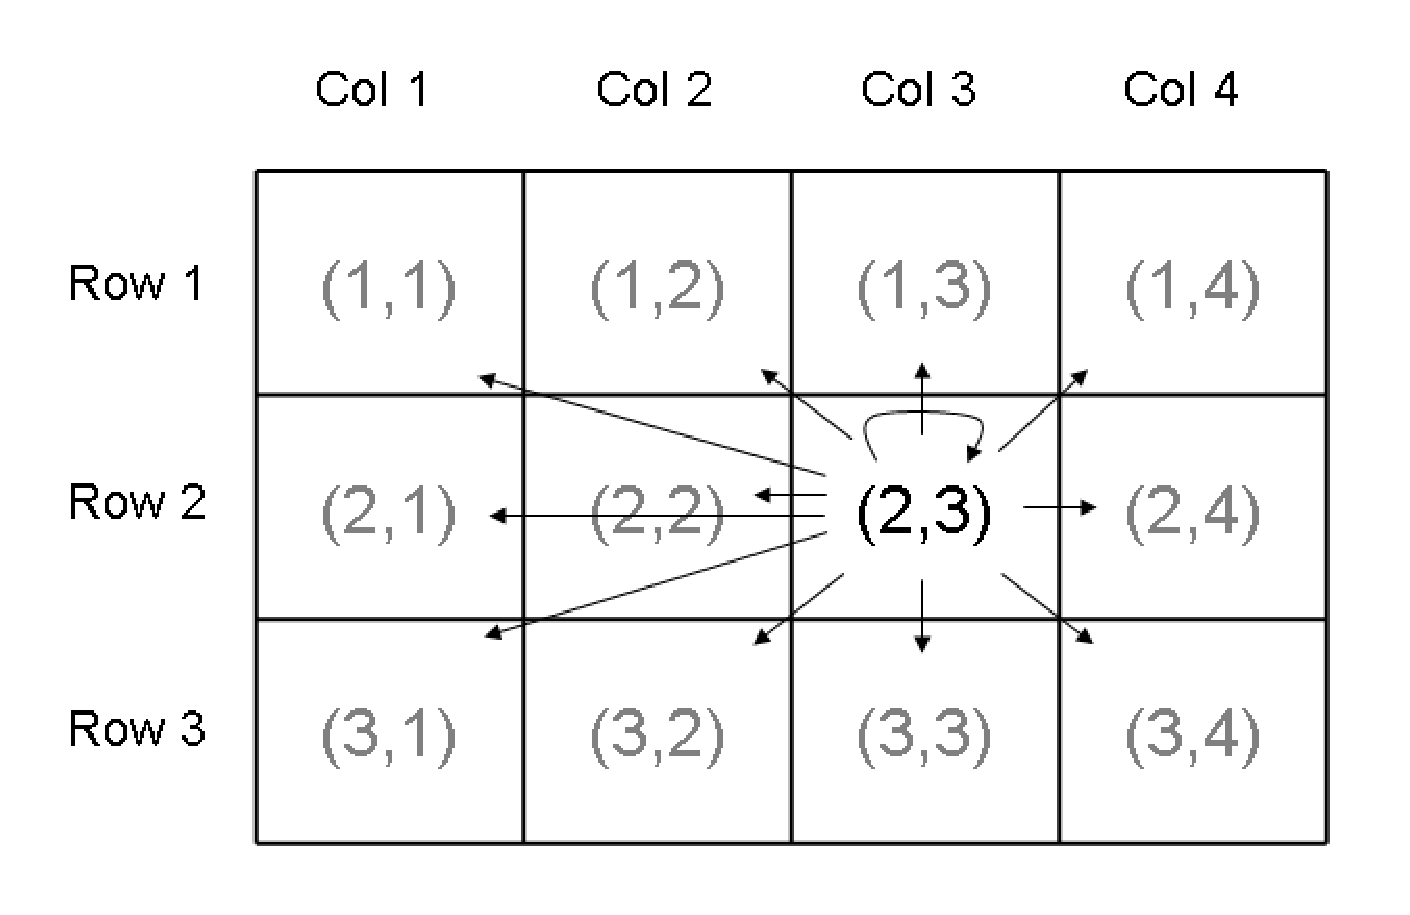
\includegraphics[width=\textwidth]{Figures/Movement}}
 \caption{Movement}
 \label{fig:Movement}
\end{figure}


\paragraph{The preference function}

 Movement in \SPM\ can be defined as a probability distribution based on an underlying preference function. Here, We define the preference for a cell $x$ as the preference function $f_x(\theta_x,P(x))$, where $\theta_x$ are the parameters for $f_x$. So, given a set of $n$ attributes for cell $x$, we can define a preference function for each, and hence we define the aggregated or total preference function for any cell $x$ as the weighted product of individual preference functions,

$P_x=f_1(\theta_1,P_1(x))^{\alpha_1} + f_2(\theta_2,P_2(x))^{\alpha_2} + f_3(\theta_3,P_3(x))^{\alpha_3} + \cdots + f_n(\theta_n,P_n(x))^{\alpha_n}$

where $\alpha_i$ is an arbitrary weighting factor for attribute $i$.

Then we define the probability of moving from cell $a$ to any cell $b$ (where $b$ is defined as the set of all possible cells, including $a$),

$p(a\rightarrow b) = {P_a} / {\sum_{i \in \forall b}P_i}$

Note that there are three forms of preference function,
\begin{enumerate}
\item Those that are a function of some underlying attribute of a cell, as defined by some arbitrary layer $L$
\item Those that are a function of the abundance (perhaps with a selectivity and for a subset of all categories) of each cell
\item Those that are a function of the distance between the sink and the source cells. 
\end{enumerate} 

Preference functions of the first type are determined only by the parameters of the preference function and some underlying, fixed, attribute. Preference functions of the other are dynamic, i.e. they depend on the relative locations of the cells or on the density of a cell at a particular point in time.

\paragraph{Preference functions}

Preference functions in \SPM\ include \subcommand{constant}, \subcommand{normal}, \subcommand{double-normal}, \subcommand{logistic}, \subcommand{inverse-logistic}, \subcommand{exponential-decay}, and \subcommand{threshold}. These are defined as,

\begin{enumerate}
\item The \subcommand{constant}\ preference function has dependent variable $x$ and has no parameters, and is defined as,

$f(x)=x$, where $0 \leq x \leq 1$

\item The \subcommand{normal}\ preference function has dependent variable $x$ and parameters $\theta = (\mu,\sigma)$, and is defined as, 

$f(x | \mu, \sigma) = 2^{-[(x- \mu)/\sigma ]^2} $
 
\item The \subcommand{double-normal}\ preference function has dependent variable $x$ and parameters $\theta=(\mu,\sigma_L,\sigma_R)$, and is defined as,

$f(x | \mu, \sigma_L, \sigma_R) = \left\{ 
\begin{array}{l l}
  2^{-[(x- \mu)/\sigma_L ]^2} & \quad \mbox{if $x \leq \mu$}\\
  2^{-[(x- \mu)/\sigma_R ]^2} & \quad \mbox{if $x \ge \mu$}\\
\end{array} \right.$ 

\item The \subcommand{logistic}\ preference function has dependent variable $x$ and parameters $\theta = (a_{50},a_{to95})$, and is defined as,

$f(x | a_{50}, a_{to95}) = 1 / [1+19^{(a_{50}-x)/a_{to95}}]$

\item The \subcommand{inverse-logistic}\ preference function has dependent variable $x$ and parameters $\theta = (a_{50},a_{to95})$, and is defined as,

$f(x | a_{50}, a_{to95}) =1- 1 / [1+19^{(a_{50}-x)/a_{to95}}]$

\item The \subcommand{exponential-decay}\ preference function has dependent variable $x$ and parameters $\theta = (\lambda)$, and is defined as,

$f(x | \lambda) =\exp(-\lambda x)$, where $x \geq 0$ and $0$ otherwise

\item The \subcommand{threshold}\ preference function has dependent variable $x$ and parameters $\theta = (N,\lambda)$, and is defined as,

$f(x | N, \lambda) = \left\{ 
\begin{array}{l l}
  1 & \quad \mbox{if $x \leq N$}\\
  1/\left({\frac{x}{N}}^\lambda\right) & \quad \mbox{if $x \ge N$}\\
\end{array} \right. $, where $x \geq 0$ and $0$ otherwise

\end{enumerate}

\subsection{Model years}

\subsection{Population processes}

\subsubsection{Recruitment}

\subsubsection{Ageing}

\subsubsection{Mortality}

\subsubsection{Category transitions}

\subsection{Movement processes}

\subsubsection{Directed movement}

\paragraph{Directed-process}

\subsection{Layers}

\subsubsection{Numeric layers}

\subsubsection{Category layers}

\subsubsection{Abundance layers}

\subsubsection{Biomass layers}

\subsubsection{Density layers}

\subsubsection{Distance layers}

\subsection{Selectivity}

\subsubsection{Logistic}

\subsubsection{Logistic producing}

\subsubsection{Knife edge}

\subsubsection{Double normal}

\subsubsection{Constant}


etc.,


\cleardoublepage{}
\section{The estimation section\label{sec:estimation-section}}

\subsection{Role of the estimation section\label{sec:role-of-the-estimation-section}}

The tasks carried out by the estimation section are: 

1. Get the point estimate, i.e., the maximum likelihood estimate (MLE) or maximum posterior density estimate (MPD) (see Section 6.3).

2. Profile selected parameters, i.e., find, for each of a series of values of a parameter, allowing the other free parameters to vary, the minimum value of the objective function (Section 6.4). This is called either a likelihood or posterior profile. 

3. For Bayesian estimation only, generate an MCMC sample from the posterior distribution (Section 6.5).

4. For maximum likelihood or Bayesian estimation, calculate the approximate covariance matrix of the parameters as the inverse of the minimiser\textquoteright{}s approximation to the Hessian, and the corresponding correlation matrix (Section 6.3).


\cleardoublepage{}
\section{The output section\label{sec:output-section}}



\cleardoublepage{}
\section{Command and subcommand syntax\label{sec:syntax}}
\subsection{General commands and subcommands\label{sec:general-syntax}}

\subsubsection{Including external files}

\defComArg{include\_file}{file\_name}{Include an external file}

\defSub{file\_name}{The name of the external file}
\defType{string}
\defDefault{None}
\defEffect{Includes an external file into the \config}
\defCondition{The file name must be enclosed in double quotes}
\defExample{\command{include\_file}{\ "my\_file.txt"}}
 

\section{Population command and subcommand syntax\label{sec:population-syntax}}

\subsection{\I{Model structure}}

\defCom{model}{Define the spatial structure, population structure, annual cycle, and model years}

\defSub{nrows}{The number of rows $n_{rows}$ in the spatial structure}
\defType{Integer}
\defDefault{No default}
\defValue{A positive integer, $n_{rows} > 0$}

\defSub{ncols}{The number of columns $n_{cols}$ in the spatial structure}
\defType{Integer}
\defDefault{No default}
\defValue{A positive integer, $n_{cols} > 0$}

\defSub{layer}{The label for the base layer}
\defType{String}
\defDefault{No default}
\defValue{Must be a label of a \argument{numeric} layer defined by \command{layer}}

\defSub{cell\_length}{The length (distance) of one side of a cell}
\defType{Constant}
\defDefault{1}
\defValue{A positive real number}

\defSub{categories} {Labels of the categories (rows) of the population component of the partition}
\defType{Vector of strings, of length $1\ldots n_{categories}$}
\defDefault{No default}
\defValue{Names of categories must be unique}

\defSub{min\_age}{Minimum age of the population}
\defType{Integer}
\defDefault{No default}
\defValue{A non-negative integer, ${age}_{min}\geq 0$ and ${age}_{min}\leq {age}_{max}$}

\defSub{max\_age}{Maximum age of the population}
\defType{Integer}
\defDefault{No default}
\defValue{A non-negative integer, ${age}_{max}\geq 0$ and ${age}_{min}\geq {age}_{min}$}

\defSub{age\_plus\_group}{Define the largest age as a plus group}
\defType{Switch}
\defDefault{True}
\defValue{Defines  the largest age as a plus group}

\defSub{age\_size}{Define the label of the associated age-size relationship for each category}
\defType{Vector of strings, of length $n_{categories}$}
\defDefault{No default}
\defValue{Must be labels of command \command{age\_size}}

\defSub{initialisation\_phases}{Define the labels of the phases of the initialisation}
\defType{Vector of strings, of length of the number of initialisation phases}
\defDefault{No default}
\defValue{A valid label defined by \command{initialisation\_phase}}

\defSub{initial\_year}{Define the first year of the model, immediately following initialisation}
\defType{Integer}
\defDefault{No default}
\defValue{Defines the first year of the model, $\geq 1$, e.g. 1990}

\defSub{current\_year}{Define the current year of the model}
\defType{Integer}
\defDefault{No default}
\defValue{Defines the current year of the model, i.e., the model is run from \commandsub{model}{first\_year}\ to \commandsub{model}{current\_year}}

%\defSub{final\_year}{Define the final year of the model in projections}
%\defType{Integer}
%\defDefault{No default}
%\defValue{Defines the final year of the model for use in projections, i.e., the model is run from \commandsub{model}{first\_year} to %\commandsub{model}{current\_year}, then projected to \commandsub{model}{final\_year}}

\defSub{time\_steps} {Define the \command{time\_step} labels (in order that they are applied) to form the annual cycle}
\defType{String vector}
\defDefault{No default}
\defValue{Defines the labels of the time-steps that are run in each year}

\subsection{\I{Initialisation}}

%The methods for initialisation available are,
%\begin{itemize}
%	\item Iterative
%\end{itemize}
%
%Each type of initialisation requires a set of subcommands and arguments specific to that type.
%
\defComLab{initialisation\_phase}{Define the processes and years of the initialisation phase with label}
%
%\defSub{type} {Define the type of initialisation}
%\defType{String}
%\defDefault{No default}
%\defValue{A valid type of initialisation}
%
%\subsubsection[Iterative initialisation]{\commandlabsubarg{initialisation\_phase}{type}{iterative}}

\defSub{years} {Define the number of years to run}
\defType{Integer}
\defDefault{No default}
\defValue{A non-negative integer}

\defSub{processes} {Define the processes (in order of occurrence) to run in each year of the initialisation}
\defType{String vector}
\defDefault{No default}
\defValue{A valid process label, from one of \command{process}}

\subsection{\I{Time-steps}}

\defComLab{time\_step} {Define a time-step with label}

\defSub{processes} {Define the process labels, in the order that they are applied, for the time-step}
\defType{String vector}
\defDefault{No default}
\defValue{Defines the labels of the processes for that time-step}

\subsection{\I{Processes}}

The population processes available are,

\begin{itemize}
	\item Constant recruitment process
  \item Beverton-Holt stock-recruit relationship recruitment process
  \item Local Beverton-Holt stock-recruit relationship recruitment process
	\item Ageing process
	\item Constant relationship mortality rate process
	\item Annually varying relationship mortality rate process
	\item Mortality event (as a number) process
	\item Mortality event (as a biomass) process
	\item Holling mortality rate
	\item Prey-switch predation process
	\item Category transition process
	\item Category shift process
\end{itemize}

The movement processes available are,

\begin{itemize}
	\item Migration movement
	\item Adjacent cell movement
	\item Preference movement
\end{itemize}

Each type of process requires a set of subcommands and arguments specific to that process.

\defComLab{process} {Define a process with label}

\defSub{type} {Define the type of process}
\defType{String}
\defDefault{No default}
\defValue{A valid type of process}

\subsubsection[Constant recruitment process]{\commandlabsubarg{process}{type}{constant\_recruitment}}

\defSub{r0} {Define the total amount of recruitment at equilibrium abundance levels}
\defType{Estimable}
\defDefault{No default}
\defValue{Total amount (in numbers) of recruitment applied across all categories at equilibrium abundances}

\defSub{categories} {Define the categories into which recruitment occurs}
\defType{String vector}
\defDefault{No default}
\defValue{Valid categories from \commandsub{model}{categories}}

\defSub{proportions} {Define the proportion of recruitment that occurs into each category}
\defType{Estimable vector, of length \subcommand{categories}}
\defDefault{No default}
\defValue{Proportion of the annual recruitment that is applied to each category}

\defSub{age} {Define the age that receives recruitment}
\defType{Integer}
\defDefault{The minimum age of the population}
\defValue{The age class that receives recruitment}

\defSub{layer} {Name of the layer used to determine where recruitment occurs}
\defType{String}
\defDefault{No default}
\defValue{A valid layer as defined by \command{layer}. If a numeric layer, then recruitment is in proportion to the layer values. Note that the layer values must be non-negative}

\subsubsection[Beverton-Holt recruitment process]{\commandlabsubarg{process}{type}{bh\_recruitment}}

\defSub{r0} {Define the total amount of recruitment at equilibrium abundance levels}
\defType{Estimable}
\defDefault{No default}
\defValue{Total amount (in numbers) of recruitment applied across all categories at equilibrium abundances}

\defSub{categories} {Define the categories into which recruitment occurs}
\defType{String vector}
\defDefault{No default}
\defValue{Valid categories from \commandsub{model}{categories}}

\defSub{proportions} {Define the proportion of recruitment that occurs into each category}
\defType{Estimable vector, of length \commandlabsub{process}{categories}}
\defDefault{No default}
\defValue{Proportion of the annual recruitment that is applied to each category}

\defSub{age} {Define the age that receives recruitment}
\defType{Integer}
\defDefault{The minimum age of the population}
\defValue{The age class that receives recruitment}

\defSub{steepness} {Define the Beverton-Holt stock recruitment relationship steepness ($h$) parameter}
\defType{Estimable}
\defDefault{1.0}
\defValue{Steepness value between 0.2 and 1.0}

%\defSub{sigma\_r} {Define the recruitment variability $\sigma_R$ in the stock-recruitment relationship for projections}
%\defType{Estimable}
%\defDefault{1.0}

%\defSub{rho} {Define the autocorrelation $\rho$ in the recruitment variability in the stock-recruitment relationship for projections}
%\defType{Estimable}
%\defDefault{0.0}

\defSub{b0} {Define the \command{initialisation\_phase} label for the value of the derived quantity  to use as the value of the spawning stock biomass ($B_0$)}
\defType{String}
\defDefault{No default}
\defValue{Must be a valid \command{initialisation\_phase} label}

\defSub{ssb} {Define the label of the \command{derived\_quantity} that defines the spawning stock biomass (SSB)}
\defType{String}
\defDefault{No default}
\defValue{Must be a valid \command{derived\_quantity} label}

\defSub{ssb\_offset} {Define the offset (in years) for the year of the derived quantity that is to be applied as the SSB in the stock-recruit relationship}
\defType{Integer}
\defDefault{No default}
\defValue{Must be a value $\ge 0$}

\defSub{ycs\_values} {YCS values}
\defType{Estimable vector}
\defDefault{No default}
\defValue{Must be vector of length \commandsub{model}{initial} to \commandsub{model}{current}}

\defSub{standardise\_ycs\_years} {Years for which the year class strength values are defined to have mean 1.0}
\defType{Integer vector or integer range}
\defDefault{No default}
\defValue{The expanded vector must have values of years between \commandsub{model}{initial} and \commandsub{model}{current}}

\defSub{layer} {Name of the layer used to determine where recruitment occurs}
\defType{String}
\defDefault{No layer}
\defValue{A valid layer as defined by \command{layer}. If a numeric layer, then recruitment is in proportion to the layer values.}

\subsubsection[Local Beverton-Holt recruitment process]{\commandlabsubarg{process}{type}{local\_bh\_recruitment}}

\defSub{r0} {Define a multiplier of \subcommand{r0\_layer} for calculating the amount of recruitment in each cell at equilibrium abundance levels}
\defType{Estimable}
\defDefault{No default}
\defValue{Multiplier of \subcommand{r0\_layer} to calculate the amount in each cell (in numbers) of recruitment applied across all categories at equilibrium abundances}

\defSub{categories} {Define the categories into which recruitment occurs}
\defType{String vector}
\defDefault{No default}
\defValue{Valid categories from \commandsub{model}{categories}}

\defSub{proportions} {Define the proportion of recruitment that occurs into each category}
\defType{Estimable vector, of length \subcommand{categories}}
\defDefault{No default}
\defValue{Proportion of the annual recruitment that is applied to each category}

\defSub{age} {Define the age that receives recruitment}
\defType{Integer}
\defDefault{No default}
\defValue{The age class that receives recruitment}

\defSub{steepness} {Define the Beverton-Holt stock recruitment relationship steepness ($h$) parameter}
\defType{Estimable}
\defDefault{1.0}
\defValue{Steepness value between 0.2 and 1.0}

%\defSub{sigma\_r} {Define the recruitment variability $\sigma_R$ in the stock-recruitment relationship for projections}
%\defType{Estimable}
%\defDefault{1.0}

%\defSub{rho} {Define the autocorrelation $\rho$ in the recruitment variability in the stock-recruitment relationship for projections}
%\defType{Estimable}
%\defDefault{0.0}

\defSub{b0} {Define the \command{initialisation\_phase} label for the value of the derived quantity  to use as the value of the spawning stock biomass ($B_0$) in each cell}
\defType{String}
\defDefault{No default}
\defValue{Must be a valid \command{initialisation\_phase} label}

\defSub{ssb} {Define the label of the \command{derived\_layer} that defines the spawning stock biomass (SSB) in each cell}
\defType{String}
\defDefault{No default}
\defValue{Must be a valid \command{derived\_layer} label}

\defSub{ssb\_offset} {Define the offset (in years) for the year of the derived layer that is to be applied as the SSB in the stock-recruit relationship}
\defType{Integer}
\defDefault{No default}
\defValue{Must be a value $\ge 0$}

\defSub{ycs\_years} {Years for year class strength values}
\defType{Integer vector or integer range}
\defDefault{No default}
\defValue{The expanded vector must be valid model years}

\defSub{ycs\_values} {YCS values}
\defType{Estimable vector}
\defDefault{No default}
\defValue{Must be vector of length \commandsub{model}{initial} to \commandsub{model}{current}}

\defSub{standardise\_ycs\_years} {Years for which the year class strength values are defined to have mean 1.0}
\defType{Integer vector or integer range}
\defDefault{No default}
\defValue{The expanded vector must have values of years between \commandsub{model}{initial} and \commandsub{model}{current}}

\defSub{layer} {Define the label of the layer that defines the distribution of recruitment (as a multpiler of $R0$ at equilibrium abundances in each cell}
\defType{String}
\defDefault{No layer}
\defValue{A valid numeric layer as defined by \command{layer}. The amount of recruitment in each cell is the product of $r0$ and the layer value in each cell.}

\subsubsection[Ageing process]{\commandlabsubarg{process}{type}{ageing}}

\defSub{categories} {Define the categories that ageing is applied to}
\defType{String vector}
\defDefault{No default}
\defValue{Valid categories from \commandsub{model}{categories}}

\subsubsection[Constant mortality rate process]{\commandlabsubarg{process}{type}{constant\_mortality\_rate}}

\defSub{m} {Define the constant mortality rate to be applied}
\defType{Estimable}
\defDefault{No default}
\defValue{A positive real number}

\defSub{categories} {Define the categories that mortality is applied to}
\defType{String vector}
\defDefault{No default}
\defValue{Valid categories from \commandsub{model}{categories}}

\defSub{selectivities} {Define the selectivities applied to each category}
\defType{String vector, of length \subcommand{categories}}
\defDefault{No default}
\defValue{Valid selectivity labels defined by \command{selectivity}}

\defSub{layer} {Name of the layer}
\defType{String}
\defDefault{No layer}
\defValue{A valid layer as defined by \command{layer}. If a numeric layer, then mortality applied is the mortality rate times the value of the layer. Note that the layer values must be non-negative}

\subsubsection[Annual mortality rate process]{\commandlabsubarg{process}{type}{annual\_mortality\_rate}}

\defSub{years} {Define the years when the mortality rates are applied}
\defType{Integer vector or integer range}
\defDefault{No default}
\defValue{Valid model years}

\defSub{m} {Define the mortality rate to be applied for each year}
\defType{Estimable vector, of length \subcommand{years} once expanded}
\defDefault{No default}
\defValue{A vector of positive real numbers}

\defSub{categories} {Define the categories that mortality is applied to}
\defType{String vector}
\defDefault{No default}
\defValue{A vector of valid categories from \commandsub{model}{categories}}

\defSub{selectivities} {Define the selectivities applied to each category}
\defType{String vector of length \subcommand{categories}}
\defDefault{No default}
\defValue{A vector of valid selectivity labels defined by \command{selectivity}}

\defSub{layer} {Name of the multiplicative layer to be applied to $M$}
\defType{String}
\defDefault{No layer}
\defValue{A valid numeric layer as defined by \command{layer}. Note that the layer values must be non-negative}

\subsubsection[Event mortality process]{\commandlabsubarg{process}{type}{event\_mortality}}

\defSub{categories} {Define the categories that the event mortality is applied to}
\defType{String vector}
\defDefault{No default}
\defValue{Valid categories from \commandsub{model}{categories}}

\defSub{years} {Define the years where the mortality even is applied}
\defType{Integer vector or integer range}
\defDefault{No default}
\defValue{Valid model years}

\defSub{layers} {Define the layers that specify the event mortality (as the abundance) in each year}
\defType{String vector, of length \subcommand{years} once expanded}
\defDefault{No default}
\defValue{Valid layers as defined by \command{layer}. Note that the layer values must be non-negative}

\defSub{u\_max}{Define the maximum exploitation rate}
\defType{Estimable}
\defDefault{0.99}
\defValue{Must be $> 0$ and $< 1$}

\defSub{selectivities} {Define the selectivities applied to each category}
\defType{String vector, of length \subcommand{categories}}
\defDefault{No default}
\defValue{Valid selectivity labels defined by \command{selectivity}}

\defSub{penalty} {Define the event mortality penalty label}
\defType{String}
\defDefault{No default}
\defValue{Valid penalty label defined by \command{penalty}}

\subsubsection[Biomass event mortality process]{\commandlabsubarg{process}{type}{biomass\_event\_mortality}}

\defSub{categories}{Define the categories that the event mortality is applied to}
\defType{String vector}
\defDefault{No default}
\defValue{Valid categories from \commandsub{model}{categories}}

\defSub{years}{Define the years where the mortality event is applied}
\defType{Integer vector or integer range}
\defDefault{No default}
\defValue{Valid years for the model}

\defSub{layers}{Define the layers that specify the event mortality (as a biomass) in each year}
\defType{String vector, of length \subcommand{years} once expanded}
\defDefault{No default}
\defValue{Valid layers defined by \command{layer}. Note that the layer values must be non-negative}

\defSub{u\_max} {Define the maximum exploitation rate}
\defType{Constant}
\defDefault{0.99}
\defValue{Must be $> 0$ and $< 1$}

\defSub{selectivities}{Define the selectivities applied to each category}
\defType{String vector, of length \subcommand{categories}}
\defDefault{No default}
\defValue{Valid selectivity labels defined by \command{selectivity}}

\defSub{penalty} {Define the event mortality penalty label}
\defType{String}
\defDefault{No default}
\defValue{Valid penalty label defined by \command{penalty}}

\subsubsection[Holling mortality rate]{\commandlabsubarg{process}{type}{Holling\_mortality\_rate}}

\defSub{is\_abundance}{Is the mortality applied as a biomass or as abundance}
\defType{Switch}
\defDefault{False}
\defValue{Either True or False}

\defSub{a}{Define the $a$ parameter of the Holling function}
\defType{Constant}
\defDefault{No default}
\defValue{A positive real number}

\defSub{b}{Define the $b$ parameter of the Holling function}
\defType{Constant}
\defDefault{No default}
\defValue{A positive real number}

\defSub{x}{Define the type of Holling function or Michaelis-Menton function}
\defType{Constant}
\defDefault{default $2$}
\defValue{A positive real number, use $2$ for Holling type II or $3$ for Holling Type III, or other positive real value for the generalised Michaelis-Menton function}

\defSub{categories}{Define the categories that the Holling mortality rate is applied to}
\defType{String vector}
\defDefault{No default}
\defValue{Valid categories from \commandsub{model}{categories}}

\defSub{selectivities}{Define the selectivities applied to each category}
\defType{String vector, of length \subcommand{categories}}
\defDefault{No default}
\defValue{Valid selectivity labels defined by \command{selectivity}}

\defSub{predator\_categories}{Define the categories of the predator}
\defType{String vector}
\defDefault{No default}
\defValue{Valid categories from \commandsub{model}{categories}}

\defSub{predator\_selectivities}{Define the selectivities applied to each predator category}
\defType{String vector, of length \subcommand{predator\_categories}}
\defDefault{No default}
\defValue{Valid selectivity labels defined by \command{selectivity}}

\defSub{u\_max} {Define the maximum exploitation rate}
\defType{Constant}
\defDefault{0.99}
\defValue{Must be $> 0$ and $< 1$}

\defSub{penalty} {Define the event mortality penalty label}
\defType{String}
\defDefault{No default}
\defValue{Valid penalty label defined by \command{penalty}}

\subsubsection[Prey-switching predation process]{\commandlabsubarg{process}{type}{Prey-switch\_predation}}

\defSub{is\_abundance}{Is the mortality applied as a biomass or as abundance}
\defType{Switch}
\defDefault{False}
\defValue{Either True or False}

\defSub{consumption\_rate}{Define the total predator consumption rate}
\defType{Numeric}
\defDefault{No default}
\defValue{A positive real number}

%\defSub{prey}{Define the vector of labels for all the prey groups used}
%\defType{String vector}
%\defDefault{No default}
%\defValue{Names must be unique}
%\defNote{These are the labels which links to the relative electivities for groups of categories}

\defSub{prey\_categories}{Define the prey categories that the predation mortality is applied to}
\defType{String vector}
\defDefault{No default}
\defValue{Valid categories from \commandsub{model}{categories}, grouping categories into $n$ prey groups using the $+$ symbol}

\defSub{prey\_selectivities}{Define the selectivities applied to each prey category}
\defType{String vector, of length \subcommand{prey\_categories}}
\defDefault{No default}
\defValue{Valid selectivity labels defined by \command{selectivity}}

\defSub{electivities}{Define the electivities applied to prey groups $1$ \ldots $n$}
\defType{Constant vector, of length $n$, the number of groups of prey in $\subcommand{prey\_categories}$}
\defDefault{No default}
\defValue{A vector of positive real numbers, must have values that sum to $1$}

%\defSub{prey\_groups}{Assign each prey category to a specific prey group}
%\defType{String vector, of length \subcommand{categories}}
%\defDefault{No default}
%\defValue{Valid labels defined by \subcommand{prey}}

\defSub{predator\_categories}{Define the categories of the predator}
\defType{String vector}
\defDefault{No default}
\defValue{Valid categories from \commandsub{model}{categories}}

\defSub{predator\_selectivities}{Define the selectivities applied to each predator category}
\defType{String vector, of length \subcommand{predator\_categories}}
\defDefault{No default}
\defValue{Valid selectivity labels defined by \command{selectivity}}

\defSub{u\_max} {Define the maximum exploitation rate}
\defType{Constant}
\defDefault{0.99}
\defValue{Must be $> 0$ and $< 1$}

\defSub{penalty} {Define the process penalty label}
\defType{String}
\defDefault{No default}
\defValue{Valid penalty label defined by \command{penalty}}

\subsubsection[Category transition process]{\commandlabsubarg{process}{type}{category\_transition}}

\defSub{from} {Define the categories that are the source of the transition process}
\defType{String vector}
\defDefault{No default}
\defValue{A valid list of categories from \commandsub{model}{categories}}

\defSub{selectivities} {Define the selectivities applied to the source categories}
\defType{String vector, of length \subcommand{from}}
\defDefault{No default}
\defValue{A valid list of selectivity labels defined by \command{selectivity}}

\defSub{to} {Define the categories that are the sink of the transition process}
\defType{String vector}
\defDefault{No default}
\defValue{A valid list of categories from \commandsub{model}{categories}}

\defSub{years} {Define the years where the category transition is applied}
\defType{Integer vector or integer range}
\defDefault{No default}
\defValue{Valid model years}

\defSub{layers} {Define the layers that specify the event mortality (as N for each cell) in each year}
\defType{String vector, of length \subcommand{years} once expanded}
\defDefault{No default}
\defValue{Valid layers defined by \command{layer}. Note that the layer values must be non-negative}

\defSub{u\_max} {Define the maximum proportion of individuals that can be moved}
\defType{Constant}
\defDefault{0.99}
\defValue{Must be $> 0$ and $\le 1$}

\defSub{penalty} {Define the penalty to encourage models parameter values away from those which result in not enough individuals to move}
\defType{String}
\defDefault{No default}
\defValue{Valid penalty label defined by \command{penalty}}

\subsubsection[Category transition rate process]{\commandlabsubarg{process}{type}{category\_transition\_rate}}

\defSub{from} {Define the category that is the source of the transition process}
\defType{String}
\defDefault{No default}
\defValue{A valid category from \commandsub{model}{categories}}

\defSub{selectivities} {Define the selectivities applied to the source categories}
\defType{String vector, of length \subcommand{from}}
\defDefault{No default}
\defValue{A valid list of selectivity labels defined by \command{selectivity}}

\defSub{to} {Define the category that is the sink of the transition process}
\defType{String}
\defDefault{No default}
\defValue{A valid category from \commandsub{model}{categories}}

\defSub{proportions} {Define the proportion of individuals to move}
\defType{Estimable}
\defDefault{No default}
\defValue{A value $\ge 0$ and $\le 1$}

\defSub{layer} {Name of the layer}
\defType{String}
\defDefault{No default}
\defValue{A valid layer as defined by \command{layer}. If a numeric layer, then rate applied to each cell is multiplied by the value of the layer. Note that the layer values must be non-negative}

\subsubsection[Migration movement]{\commandlabsubarg{process}{type}{migration}}

\defSub{categories} {Define the categories that the migration movement event is applied to}
\defType{String vector}
\defDefault{No default}
\defValue{Valid categories from \commandsub{model}{categories}}

\defSub{selectivities} {Define the selectivities applied to each category}
\defType{String vector, of length \subcommand{categories}}
\defDefault{No default}
\defValue{Valid selectivity labels defined by \command{selectivity}}

\defSub{proportion} {Define the constant multiplier for the proportion of individuals that migrate}
\defType{Estimable}
\defDefault{1.0}
\defValue{A real number between 0 and 1, inclusive}

\defSub{source\_layer} {Define the label of a layer that defines the source cells of the migration movement event}
\defType{String}
\defDefault{No default}
\defValue{A valid layer defined by \command{layer}}

\defSub{sink\_layer} {Define the label of a layer that defines the sink cells of the migration movement event}
\defType{String}
\defDefault{No default}
\defValue{A valid layer defined by \command{layer}}

\subsubsection[Adjacent cell movement]{\commandlabsubarg{process}{type}{adjacent\_cell}}

\defSub{categories} {Define the categories that the adjacent cell movement event is applied to}
\defType{String vector}
\defDefault{No default}
\defValue{Valid categories from \commandsub{model}{categories}}

\defSub{selectivities} {Define the selectivities applied to each category}
\defType{String vector, of length \subcommand{categories}}
\defDefault{No default}
\defValue{Valid selectivity labels defined by \command{selectivity}}

\defSub{layer} {Define the label of a gradient layer that defines the the relative strength of movement to adjacent cells}
\defType{String}
\defDefault{Default 1 in every cell, equivalent to uniform diffusion}
\defValue{A valid layer defined by \command{layer}}

\defSub{proportion} {Define the constant multiplier for the proportion that moves from each cell to the neighbouring cell}
\defType{Estimable}
\defDefault{1.0}
\defValue{A real number between 0 and 1, inclusive}

\subsubsection[Preference movement]{\commandlabsubarg{process}{type}{preference}}

\defSub{categories} {Define the categories that the preference function movement is applied to}
\defType{String vector}
\defDefault{No default}
\defValue{Valid categories from \commandsub{model}{categories}}

\defSub{proportion} {Define the constant multiplier for the proportion that the preference function movement is applied to}
\defType{Estimable}
\defDefault{1.0}
\defValue{A real number between 0 and 1, inclusive}

\defSub{preference\_functions} {Define the labels of the individual  preference functions that make up the total preference function}
\defType{String vector}
\defDefault{No default}
\defValue{Valid preference function labels defined by \command{preference\_function}}

\subsection{\I{Preference functions}}

The individual preference functions available are,

\begin{itemize}
	\item Constant
	\item Normal
	\item Double normal
	\item Logistic
	\item Inverse logistic
	\item Exponential
	\item Threshold
	\item Categorical
	\item Monotonic categorical
\end{itemize}

Each type of preference function requires a set of subcommands and arguments specific to that function.

\defComLab{preference\_function} {Define a preference function with label}

\defSub{type} {Define the type of preference function}
\defType{String}
\defDefault{No default}
\defValue{A valid type of preference function}

\subsubsection[Constant]{\commandlabsubarg{preference\_function}{type}{constant}}

\defSub{layer} {Defines the layer which supplies the preference function independent variable}
\defType{String}
\defDefault{No default}
\defValue{A valid layer defined by \command{layer}}

\defSub{alpha} {Defines the multiplicative constant $\alpha$}
\defType{Estimable}
\defDefault{No default}

\subsubsection[Normal]{\commandlabsubarg{preference\_function}{type}{normal}}

\defSub{layer} {Defines the layer which supplies the preference function independent variable}
\defType{String}
\defDefault{No default}
\defValue{A valid layer defined by \command{layer}}

\defSub{alpha} {Defines the multiplicative constant $\alpha$}
\defType{Estimable}
\defDefault{No default}

\defSub{mu} {Defines the $\mu$ parameter of the normal preference function}
\defType{Estimable}
\defDefault{No default}

\defSub{sigma} {Defines the $\sigma$ parameter of the normal preference function}
\defType{Estimable}
\defDefault{No default}

\subsubsection[Double-normal]{\commandlabsubarg{preference\_function}{type}{double\_normal}}

\defSub{layer} {Defines the layer which supplies the preference function independent variable}
\defType{String}
\defDefault{No default}
\defValue{A valid layer defined by \command{layer}}

\defSub{alpha} {Defines the multiplicative constant $\alpha$}
\defType{Estimable}
\defDefault{No default}

\defSub{mu} {Defines the $\mu$ parameter of the double-normal preference function}
\defType{Estimable}
\defDefault{No default}

\defSub{sigma\_l} {Defines the $\sigma_L$ parameter of the double-normal preference function}
\defType{Estimable}
\defDefault{No default}

\defSub{sigma\_r} {Defines the $\sigma_R$ parameter of the double-normal preference function}
\defType{Estimable}
\defDefault{No default}

\subsubsection[Logistic]{\commandlabsubarg{preference\_function}{type}{logistic}}

\defSub{layer} {Defines the layer which supplies the preference function independent variable}
\defType{String}
\defDefault{No default}
\defValue{A valid layer defined by \command{layer}, with strictly positive values only}

\defSub{alpha} {Defines the multiplicative constant $\alpha$}
\defType{Estimable}
\defDefault{No default}

\defSub{a50} {Defines the $a_{50}$ parameter of the logistic preference function}
\defType{Estimable}
\defDefault{No default}

\defSub{ato95} {Defines the $a_{to95}$ parameter of the logistic preference function}
\defType{Estimable}
\defDefault{No default}

\subsubsection[Inverse-logistic]{\commandlabsubarg{preference\_function}{type}{inverse\_logistic}}

\defSub{layer} {Defines the layer which supplies the preference function independent variable}
\defType{String}
\defDefault{No default}
\defValue{A valid layer defined by \command{layer}, with strictly positive values only}

\defSub{alpha} {Defines the multiplicative constant $\alpha$}
\defType{Estimable}
\defDefault{No default}

\defSub{a50} {Defines the $a_{50}$ parameter of the inverse-logistic preference function}
\defType{Estimable}
\defDefault{No default}

\defSub{ato95} {Defines the $a_{to95}$ parameter of the inverse-logistic preference function}
\defType{Estimable}
\defDefault{No default}

\subsubsection[Exponential]{\commandlabsubarg{preference\_function}{type}{exponential}}

\defSub{layer} {Defines the layer which supplies the preference function independent variable}
\defType{String}
\defDefault{No default}
\defValue{A valid layer defined by \command{layer} of positive values only}

\defSub{alpha} {Defines the multiplicative constant $\alpha$}
\defType{Estimable}
\defDefault{No default}

\defSub{lambda} {Defines the $\lambda$ parameter of the exponential preference function}
\defType{Estimable}
\defDefault{No default}

\subsubsection[Threshold]{\commandlabsubarg{preference\_function}{type}{threshold}}

\defSub{layer} {Defines the layer which supplies the preference function independent variable}
\defType{String}
\defDefault{No default}
\defValue{A valid layer defined by \command{layer}}

\defSub{alpha} {Defines the multiplicative constant $\alpha$}
\defType{Estimable}
\defDefault{No default}

\defSub{n} {Defines the $N$ parameter of the threshold preference function}
\defType{Estimable}
\defDefault{No default}

\defSub{lambda} {Defines the $\lambda$ parameter of the threshold preference function}
\defType{Estimable}
\defDefault{No default}

\subsubsection[Categorical]{\commandlabsubarg{preference\_function}{type}{categorical}}

\defSub{layer} {Defines the layer which supplies the preference function independent variable}
\defType{String}
\defDefault{No default}
\defValue{A valid layer defined by \command{layer}}

\defSub{alpha} {Defines the multiplicative constant $\alpha$}
\defType{Estimable}
\defDefault{No default}

\defSub{category\_labels} {Defines the unique labels of \argument{layer} in order of their coefficients}
\defType{String vector}
\defDefault{No default}
\defValue{A complete set of unique values of labels in \argument{layer} in order of \argument{category\_values}}

\defSub{category\_values} {Defines the coefficients for each unique label of \argument{layer} in order of their labels}
\defType{String vector}
\defDefault{No default}
\defValue{A complete set of positive values of labels in \argument{layer} in order of \argument{category\_labels}}

\subsubsection[Monotonic categorical]{\commandlabsubarg{preference\_function}{type}{monotonic\_categorical}}

\defSub{layer} {Defines the layer which supplies the preference function independent variable}
\defType{String}
\defDefault{No default}
\defValue{A valid layer defined by \command{layer}}

\defSub{alpha} {Defines the multiplicative constant $\alpha$}
\defType{Estimable}
\defDefault{No default}

\defSub{category\_labels} {Defines the unique labels of \argument{layer} in order of their coefficients}
\defType{String vector}
\defDefault{No default}
\defValue{A complete set of unique values of labels in \argument{layer} in order of \argument{category\_values}}

\defSub{category\_values} {Defines the coefficients for each unique label of \argument{layer} in order of their labels}
\defType{Numeric vector}
\defDefault{No default}
\defValue{A complete set of positive values of labels in \argument{layer} in order of \argument{category\_labels}}

\subsection{\I{Layers}}

The available layer types  are,

\begin{itemize}
	\item Numeric
	\item Categorical
	\item Distance
	\item Abundance
	\item Biomass
	\item Abundance density
	\item Biomass density
	\item Numeric meta-layer
	\item Categorical meta-layer
\end{itemize}

\defComLab{layer} {Define a layer function with label}

\defSub{type} {Define the type of layer}
\defType{String}
\defDefault{No default}
\defValue{A valid type of layer}

\subsubsection[Numeric]{\commandlabsubarg{layer}{type}{numeric}}

\defSub{data} {Define the values of the layer}
\defType{Constant vector, with total length \commandsub{model}{ncols} $\times$ \commandsub{model}{nrows}}
\defDefault{No default}
\defValue{A vector of values of length equal to the number of elements defined for the spatial structure}

\subsubsection[Categorical]{\commandlabsubarg{layer}{type}{categorical}}

\defSub{data} {Define the values of the layer}
\defType{Constant vector, with total length \commandsub{model}{ncols} $\times$ \commandsub{model}{nrows}}
\defDefault{No default}
\defValue{A vector of values of length equal to the number of elements defined for the spatial structure}

\subsubsection[Distance]{\commandlabsubarg{layer}{type}{distance}}

There are no other subcommands for \commandlabsubarg{layer}{type}{distance}.

\subsubsection[Abundance]{\commandlabsubarg{layer}{type}{abundance}}

\defSub{categories} {Define the categories are used to calculate the abundance}
\defType{String vector}
\defDefault{No default}
\defValue{Valid categories from \commandsub{model}{categories}}

\defSub{selectivities} {Define the selectivities applied to each category}
\defType{String vector, of length \subcommand{categories}}
\defDefault{No default}
\defValue{Valid selectivity labels from \command{selectivity}}

\subsubsection[Biomass]{\commandlabsubarg{layer}{type}{biomass}}

\defSub{categories} {Define the categories are used to calculate the biomass}
\defType{String vector}
\defDefault{No default}
\defValue{Valid categories from \commandsub{model}{categories}}

\defSub{selectivities} {Define the selectivities applied to each category}
\defType{String vector, of length \subcommand{categories}}
\defDefault{No default}
\defValue{Valid selectivity labels from \command{selectivity}}

\subsubsection[Abundance-density]{\commandlabsubarg{layer}{type}{abundance\_density}}

\defSub{categories} {Define the categories are used to calculate the abundance}
\defType{String vector}
\defDefault{No default}
\defValue{Valid categories from \commandsub{model}{categories}}

\defSub{selectivities} {Define the selectivities applied to each category}
\defType{String vector, of length \subcommand{categories}}
\defDefault{No default}
\defValue{Valid selectivity labels from \command{selectivity}}

\subsubsection[Biomass-density]{\commandlabsubarg{layer}{type}{biomass\_density}}

\defSub{categories} {Define the categories are used to calculate the biomass}
\defType{String vector}
\defDefault{No default}
\defValue{Valid categories from \commandsub{model}{categories}}

\defSub{selectivities} {Define the selectivities applied to each category}
\defType{String vector, of length \subcommand{categories}}
\defDefault{No default}
\defValue{Valid selectivity labels from \command{selectivity}}

\subsubsection[Numeric meta-layer]{\commandlabsubarg{layer}{type}{numeric\_meta}}

\defSub{default\_layer} {Define the default layer to use in years or initialisation phases where it is not otherwise defined}
\defType{String}
\defDefault{No default}
\defCondition{The argument must be a numeric layer}

\defSub{years} {Define the years that have a non-default layer}
\defType{Integer vector or integer range}
\defDefault{No default}
\defValue{Must be valid model years}

\defSub{layers} {Define the layers for each of the years}
\defType{String vector, of length \argument{year} once expanded}
\defDefault{No default}
\defCondition{The arguments must be numeric layers}

\defSub{initialisation\_phases} {Define the initialisation phases that have a non-default layer}
\defType{String vector}
\defDefault{No default}
\defCondition{The arguments must be numeric layers}

\defSub{initialisation\_layers} {Define the layers for each of the initialisation phases}
\defType{String vector, of length the number of \argument{initialisation\_phases}}
\defDefault{No default}
\defCondition{The arguments must be numeric layers}

\subsubsection[Categorical meta-layer]{\commandlabsubarg{layer}{type}{categorical\_meta}}

\defSub{default\_layer} {Define the default layer to use in years or initialisation phases where it is not otherwise defined}
\defType{String}
\defDefault{No default}
\defCondition{The argument must be a categorical layer}

\defSub{years} {Define the years that have a non-default layer}
\defType{Integer vector or integer range}
\defDefault{No default}
\defValue{Must be valid model years}

\defSub{layers} {Define the layers for each of the years}
\defType{String vector, of length \argument{year} once expanded}
\defDefault{No default}
\defCondition{The arguments must be categorical layers}

\defSub{initialisation\_phases} {Define the initialisation phases that have a non-default layer}
\defType{String vector}
\defDefault{No default}
\defCondition{The arguments must be categorical layers}

\defSub{initialisation\_layers} {Define the layers for each of the initialisation phases}
\defType{String vector, of length the number of \argument{initialisation\_phases}}
\defDefault{No default}
\defCondition{The arguments must be categorical layers}

\subsection{\I{Derived layers}}

The individual types of derived layers available are,

\begin{itemize}
	\item Abundance
	\item Biomass
\end{itemize}

\defComLab{derived\_layer} {Define a derived layer with label}

\defSub{type} {Define the type of derived layer}
\defType{String}
\defDefault{No default}
\defValue{A valid type of derived layer, either \texttt{abundance} or \texttt{biomass}}

\subsubsection[Abundance]{\commandlabsubarg{derived\_layer}{type}{abundance}}

\defSub{categories} {Define the categories are used to calculate the derived layer}
\defType{String vector}
\defDefault{No default}
\defValue{Valid categories from \commandsub{model}{categories}}

\defSub{selectivities} {Define the selectivities}
\defType{String vector, of length \subcommand{categories}}
\defDefault{No default}
\defValue{Valid selectivity labels from \command{selectivity}}

\defSub{initialisation\_time\_steps} {Define the time-steps during the initialisation phases at the end of which the derived layer is calculated}
\defType{String}
\defDefault{No default}
\defValue{A valid time-step label from \command{time\_step}}

\defSub{time\_step} {Define the time-step at the end of which the derived layer is calculated}
\defType{String}
\defDefault{No default}
\defValue{A valid time-step label from \command{time\_step}}

\defSub{layer} {Define the layer to be used in the calculations}
\defType{String}
\defDefault{None}
\defValue{A valid numeric layer as defined by \command{layer}. Note, the final value of the derived layer is the sum of the each cell is multiplied by the value of this layer.}

\subsubsection[Biomass]{\commandlabsubarg{derived\_layer}{type}{biomass}}

\defSub{categories} {Define the categories are used to calculate the derived layer}
\defType{String vector}
\defDefault{No default}
\defValue{Valid categories from \commandsub{model}{categories}}

\defSub{selectivities} {Define the selectivities}
\defType{String vector, of length \subcommand{categories}}
\defDefault{No default}
\defValue{Valid selectivity labels from \command{selectivity}}

\defSub{initialisation\_time\_steps} {Define the time-steps during the initialisation phases at the end of which the derived layer is calculated}
\defType{String}
\defDefault{No default}
\defValue{A valid time-step label from \command{time\_step}}

\defSub{time\_step} {Define the time-step at the end of which the derived layer is calculated}
\defType{String}
\defDefault{No default}
\defValue{A valid time-step label from \command{time\_step}}

\defSub{layer} {Define the layer to be used in the calculations}
\defType{String}
\defDefault{None}
\defValue{A valid numeric layer as defined by \command{layer}. Note, the final value of the derived layer is the sum of the each cell is multiplied by the value of this layer.}

\subsection{\I{Derived quantities}}

The individual types of derived quantities available are,

\begin{itemize}
	\item Abundance
	\item Biomass
\end{itemize}

\defComLab{derived\_quantity} {Define a derived quantity with label}

\defSub{type} {Define the type of derived quantity}
\defType{String}
\defDefault{No default}
\defValue{A valid type of derived quantity, either \texttt{abundance} or \texttt{biomass}}

\subsubsection[Abundance]{\commandlabsubarg{derived\_quantity}{type}{abundance}}

\defSub{categories} {Define the categories are used to calculate the derived quantity}
\defType{String vector}
\defDefault{No default}
\defValue{Valid categories from \commandsub{model}{categories}}

\defSub{selectivities} {Define the selectivities}
\defType{String vector, of length \subcommand{categories}}
\defDefault{No default}
\defValue{Valid selectivity labels from \command{selectivity}}

\defSub{initialisation\_time\_steps} {Define the time-steps during the initialisation phases at the end of which the derived quantity is calculated}
\defType{String}
\defDefault{No default}
\defValue{A valid time-step label from \command{time\_step}}

\defSub{time\_step} {Define the time-step at the end of which the derived quantity is calculated}
\defType{String}
\defDefault{No default}
\defValue{A valid time-step label from \command{time\_step}}

\defSub{layer} {Define the layer to be used in the calculations}
\defType{String}
\defDefault{None}
\defValue{A valid numeric layer as defined by \command{layer}. Note, the final value of the derived quantity is the sum of the each cell is multiplied by the value of this layer.}

\subsubsection[Biomass]{\commandlabsubarg{derived\_quantity}{type}{biomass}}

\defSub{categories} {Define the categories are used to calculate the derived quantity}
\defType{String vector}
\defDefault{No default}
\defValue{Valid categories from \commandsub{model}{categories}}

\defSub{selectivities} {Define the selectivities}
\defType{String vector, of length \subcommand{categories}}
\defDefault{No default}
\defValue{Valid selectivity labels from \command{selectivity}}

\defSub{initialisation\_time\_steps} {Define the time-steps during the initialisation phases at the end of which the derived quantity is calculated}
\defType{String}
\defDefault{No default}
\defValue{A valid time-step label from \command{time\_step}}

\defSub{time\_step} {Define the time-step at the end of which the derived quantity is calculated}
\defType{String}
\defDefault{No default}
\defValue{A valid time-step label from \command{time\_step}}

\defSub{layer} {Define the layer to be used in the calculations}
\defType{String}
\defDefault{None}
\defValue{A valid numeric layer as defined by \command{layer}. Note, the final value of the derived layer is the sum of the each cell is multiplied by the value of this layer.}

\subsection{\I{Age-size relationship}}

The individual types of size-at-age relationships available are,

\begin{itemize}
	\item none
	\item von Bertalanffy
	\item Schnute
\end{itemize}

\defComLab{age\_size} {Define an age-size relationship with label}

\defSub{type} {Define the type of size-at-age relationship}
\defType{String}
\defDefault{No default}
\defValue{A valid type of size-at-age relationship}

\subsubsection[von Bertalanffy]{\commandlabsubarg{age\_size}{type}{von\_bertalanffy}}

\defSub{linf} {Define the $L_\infty$ parameter of the von Bertalanffy relationship}
\defType{Estimable}
\defDefault{No default}
\defValue{A positive real number}
\defCondition{Only define if using the von Bertalanffy relationship}

\defSub{k} {Define the $k$ parameter of the von Bertalanffy relationship}
\defType{Estimable}
\defDefault{No default}
\defValue{A positive real number}
\defCondition{Only define if using the von Bertalanffy relationship}

\defSub{t0} {Define the $t_0$ parameter of the von Bertalanffy relationship}
 \defType{Estimable}
\defDefault{No default}
\defValue{A real number}
\defCondition{Only define if using the von Bertalanffy relationship}

%\defSub{distribution} {Define the distribution of sizes-at-age around the mean}
%\defType{String}
%\defDefault{Normal}
%\defValue{Either normal or lognormal}
%\defCondition{Only define if using the von Bertalanffy relationship}
%
%\defSub{by\_length} {Specifies if the linear interpolation of c.v.s is a linear function of mean size or of age}
%\defType{Logical}
%\defDefault{True}
%\defValue{If true, the the c.v. is a function of length, else a function of age}
%
%\defSub{cv} {Define the c.v. of the distribution of sizes-at-age around the mean}
%\defType{Estimable}
%\defDefault{No default}
%\defValue{A positive real number}
%
%\defSub{growth\_proportions} {Define the proportion of the year for each time-step for evaluating size}
%\defType{Constant vector}
%\defDefault{No default}
%\defValue{A vector of values, $\le1$ of length equal to the number of time-steps}
%
\defSub{size\_weight} {Define the label of the associated size-weight relationship}
\defType{String}
\defDefault{No default}
\defValue{A valid label from \command{size\_weight}}

\subsubsection[Schnute]{\commandlabsubarg{age\_size}{type}{schnute}}

\defSub{y1} {Define the $y_1$ parameter of the Schnute relationship}
\defType{Estimable}
\defDefault{No default}
\defValue{A positive real number}
\defCondition{Only define if using the Schnute relationship}

\defSub{y2} {Define the $y_2$ parameter of the Schnute relationship}
\defType{Estimable}
\defDefault{No default}
\defValue{A positive real number}
\defCondition{Only define if using the Schnute relationship}

\defSub{tau1} {Define the $\tau_1$ parameter of the Schnute relationship}
\defType{Estimable}
\defDefault{No default}
\defValue{A real number}
\defCondition{Only define if using the Schnute relationship}

\defSub{tau2} {Define the $\tau_2$ parameter of the Schnute relationship}
\defType{String}
\defDefault{Normal}
\defValue{Either normal or lognormal}
\defCondition{Only define if using the Schnute relationship}

\defSub{a} {Define the $a$ parameter of the Schnute relationship}
\defType{String}
\defDefault{Normal}
\defValue{Either normal or lognormal}
\defCondition{Only define if using the Schnute relationship}

\defSub{b} {Define the $b$ parameter of the Schnute relationship}
\defType{String}
\defDefault{Normal}
\defValue{Either normal or lognormal}
\defCondition{Only define if using the Schnute relationship}

%\defSub{by\_length} {Specifies if the linear interpolation of c.v.s is a linear function of mean size or of age}
%\defType{Logical}
%\defDefault{True}
%\defValue{If true, the the c.v. is a function of length, else a function of age}
%
%\defSub{cv} {Define the c.v. of the distribution of sizes-at-age around the mean}
%\defType{Estimable}
%\defDefault{No default}
%\defValue{A positive real number}
%
%\defSub{growth\_proportions} {Define the proportion of the year for each time-step for evaluating size}
%\defType{Constant vector}
%\defDefault{No default}
%\defValue{A vector of values, $\le1$ of length equal to the number of time-steps}
%
\defSub{size\_weight} {Define the label of the associated size-weight relationship}
\defType{String}
\defDefault{No default}
\defValue{A valid label from \command{size\_weight}}

\subsection{\I{Size-weight}}

The individual types of size-weight relationship available are,

\begin{itemize}
	\item None
	\item Basic
\end{itemize}

\defComLab{size\_weight} {Define a size-weight relationship with label}

\defSub{type} {Define the type of relationship}
\defType{String}
\defDefault{No default}
\defValue{A valid type of size-weight relationship}

\subsubsection[None]{\commandlabsubarg{size\_weight}{type}{none}}

There are no other subcommands for \commandlabsubarg{size\_weight}{type}{none}.

\subsubsection[Basic]{\commandlabsubarg{size\_weight}{type}{basic}}

\defSub{a} {Define the $a$ parameter of the basic size-weight relationship}
\defType{Estimable}
\defDefault{No default}
\defValue{A positive real number}

\defSub{b} {Define the $b$ parameter of the basic size-weight relationship}
\defType{Estimable}
\defDefault{No default}
\defValue{A positive real number}

\subsection{\I{Selectivities}}

The individual selectivity functions available are,

\begin{itemize}
	\item Constant
	\item Knife edge
	\item All values
	\item All values bounded
	\item Increasing
	\item Logistic
	\item Inverse Logistic
	\item Logistic producing
	\item Double normal
	\item Double exponential
\end{itemize}

Each type of selectivity function requires a set of subcommands and arguments specific to that function.

\defComLab{selectivity} {Define a selectivity function with label}

\defSub{type} {Define the type of selectivity function}
\defType{String}
\defDefault{No default}
\defValue{A valid type of selectivity function}

\subsubsection[Constant]{\commandlabsubarg{selectivity}{type}{constant}}

\defSub{c} {Defines the $C$ parameter of the selectivity function}
\defType{Estimable}
\defDefault{No default}
\defValue{A positive real number}

\subsubsection[Knife-edge]{\commandlabsubarg{selectivity}{type}{knife\_edge}}

\defSub{e} {Defines the $E$ parameter of the selectivity function}
\defType{Estimable}
\defDefault{No default}
\defValue{A positive real number}

\subsubsection[All-values]{\commandlabsubarg{selectivity}{type}{all\_values}}

\defSub{v} {Defines the $V$ parameters (one for each age class) of the selectivity function}
\defType{Estimable vector}
\defDefault{No default}
\defValue{A vector of positive real numbers, of length equal to the number of age classes}

\subsubsection[All-values-bounded]{\commandlabsubarg{selectivity}{type}{all\_values\_bounded}}

\defSub{l} {Defines the $L$ parameter of the selectivity function}
\defType{Integer}
\defDefault{No default}
\defValue{A positive real number}

\defSub{h} {Defines the $H$ parameter of the selectivity function}
\defType{Integer}
\defDefault{No default}
\defValue{A positive real number, must be greater than $L$}

\defSub{v} {Defines the $V$ parameters (one for each age class from $L$ to $H$) of the selectivity function}
\defType{Estimable vector}
\defDefault{No default}
\defValue{A vector of positive real numbers, of length equal to the number of age classes from $L$ to $H$}

\subsubsection[Increasing]{\commandlabsubarg{selectivity}{type}{increasing}}

\defSub{alpha} {Defines the $\alpha$ parameter of the selectivity function}
\defType{Estimable}
\defDefault{No default}
\defValue{A positive real number}

\defSub{l} {Defines the $L$ parameter of the selectivity function}
\defType{Integer}
\defDefault{No default}
\defValue{A positive real number}

\defSub{h} {Defines the $H$ parameter of the selectivity function}
\defType{Integer}
\defDefault{No default}
\defValue{A positive real number, must be greater than $L$}

\defSub{v} {Defines the $V$ parameters (one for each age class from $L$ to $H$) of the selectivity function}
\defType{Estimable vector}
\defDefault{No default}
\defValue{A vector of positive real numbers, of length equal to the number of age classes from $L$ to $H$}

\subsubsection[Logistic]{\commandlabsubarg{selectivity}{type}{logistic}}

\defSub{alpha} {Defines the $\alpha$ parameter of the selectivity function}
\defType{Estimable}
\defDefault{No default}
\defValue{A positive real number}

\defSub{a50} {Defines the $a_{50}$ parameter of the selectivity function}
\defType{Estimable}
\defDefault{No default}
\defValue{A positive real number}

\defSub{ato95} {Defines the $a_{to95}$ parameter of the selectivity function}
\defType{Estimable}
\defDefault{No default}
\defValue{A positive real number}

\subsubsection[InverseLogistic]{\commandlabsubarg{selectivity}{type}{inverse\_logistic}}

\defSub{alpha} {Defines the $\alpha$ parameter of the selectivity function}
\defType{Estimable}
\defDefault{No default}
\defValue{A positive real number}

\defSub{a50} {Defines the $a_{50}$ parameter of the selectivity function}
\defType{Estimable}
\defDefault{No default}
\defValue{A positive real number}

\defSub{ato95} {Defines the $a_{to95}$ parameter of the selectivity function}
\defType{Estimable}
\defDefault{No default}
\defValue{A positive real number}

\subsubsection[Logistic producing]{\commandlabsubarg{selectivity}{type}{logistic\_producing}}

\defSub{alpha} {Defines the $\alpha$ parameter of the selectivity function}
\defType{Estimable}
\defDefault{No default}
\defValue{A positive real number}

\defSub{l} {Defines the $L$ parameter of the selectivity function}
\defType{Integer}
\defDefault{No default}
\defValue{A positive real number}

\defSub{h} {Defines the $H$ parameter of the selectivity function}
\defType{Integer}
\defDefault{No default}
\defValue{A positive real number, must be greater than $L$}

\defSub{a50} {Defines the $a_{50}$ parameter of the selectivity function}
\defType{Estimable}
\defDefault{No default}
\defValue{A positive real number}

\defSub{ato95} {Defines the $a_{to95}$ parameter of the selectivity function}
\defType{Estimable}
\defDefault{No default}
\defValue{A positive real number}

\subsubsection[Double-normal]{\commandlabsubarg{selectivity}{type}{double\_normal}}

\defSub{alpha} {Defines the $\alpha$ parameter of the selectivity function}
\defType{Estimable}
\defDefault{No default}
\defValue{A positive real number}

\defSub{mu} {Defines the $\mu$ parameter of the selectivity function}
\defType{Estimable}
\defDefault{No default}

\defSub{sigma\_l} {Defines the $\sigma_L$ parameter of the selectivity function}
\defType{Estimable}
\defDefault{No default}

\defSub{sigma\_r} {Defines the $\sigma_R$ parameter of the selectivity function}
\defType{Estimable}
\defDefault{No default}

\subsubsection[Double-exponential]{\commandlabsubarg{selectivity}{type}{double\_exponential}}

\defSub{alpha} {Defines the $\alpha$ parameter of the selectivity function}
\defType{Estimable}
\defDefault{No default}
\defValue{A positive real number}

\defSub{x1} {Defines the $x_1$ parameter of the selectivity function}
\defType{Integer}
\defDefault{No default}

\defSub{x2} {Defines the $x_2$ parameter of the selectivity function}
\defType{Integer}
\defDefault{No default}

\defSub{x0} {Defines the $x_0$ parameter of the selectivity function}
\defType{Estimable}
\defDefault{No default}

\defSub{y0} {Defines the $y_0$ parameter of the selectivity function}
\defType{Estimable}
\defDefault{No default}

\defSub{y1} {Defines the $y_1$ parameter of the selectivity function}
\defType{Estimable}
\defDefault{No default}

\defSub{y2} {Defines the $y_2$ parameter of the selectivity function}
\defType{Estimable}
\defDefault{No default}

%Not implemented yet. A way to apply joint selectivity would be to arbitrarily fix the first selectivity to one and only estimate the second one (say using a pointer?). If the estimated selectivity is above 1, it gets fixed to 1 and the other one gest estimated. Both get reported.
%
%\defComLab{joint\_selectivity} {Define a joint selectivity}
%
%\defSub{selectivities} {Define the labels of the selectivities to be defined as 'joint'}
%\defType{String vector of length 2}
%\defDefault{No default}
%\defValue{Valid \command{selectivity} labels}

\section{Estimation command and subcommand syntax\label{sec:estimation-syntax}}


\section{Output command and subcommand syntax\label{sec:output-syntax}}

\subsection{Free parameters\label{sec:InputFileFormat}}



\cleardoublepage{}

\section{Examples\label{sec:examples}}


\subsection{Simple 1x1 spatial structure example\label{example1}}


\subsection{Complex 10x10 spatial structure example\label{example2}}



\cleardoublepage{}
\section{Post processing output using \R \label{sec:post-processing}}

The \R\ package \texttt{spm} contains a set of \R\ functions for reading \SPM\ output, and is available as a precompiled binary for Microsoft Windows (.zip file) or as a source package (.gz file) for Linux. To check the version number and date of the \texttt{spm} \R\ package (useful for checking that you have the most recent version), use the function \texttt{spm.version()}.

The \texttt{spm} \R\ package includes a range of extract and write functions to aid post-processing of \SPM\ \config s and output. The main extract functions are briefly described below. In addition, the package also some undocumented helper functions, that could be useful for writing you own analysis functions. See the the \R\ help for more detail e.g., \texttt{help(spm)}

\subsection{Read and extract reports from a SPM output file.}

Command: \texttt{extract()} 

Usage: \texttt{extract(file, path = "", ignore.unknown=FALSE)}

Arguments:
\begin{description}
\item[\texttt{file}] the name of the SPM output file to read
\item[\texttt{path}] Optionally, the operating system path to the directory of the output file.
\item[\texttt{ignore.unknown}] Ignore unknown reports when reading. (This can be useful to read files that contain undocumented reports or other output)
\end{description}

Output: A list object with elements for each report type.


\cleardoublepage{}
\section{Changes and enhancements from previous versions}


\subsection{Introduction}

The changes and enhancements between published versions \SPM are detailed below. These include any incremental changes for unpublished version that may have been distributed between published versions. 


\cleardoublepage{}
\section{Troubleshooting\label{sec:trouble-shooting}}

\subsection{Introduction}

\SPM\ is a complex system, providing many opportunities for error --- either because the parameter files do not correctly specify the model, or because the model specified does not work as expected. When in doubt, ask an experienced user. Debugging versions of \SPM\ can also be compiled that help to track down cryptic errors.

When \SPM\ generates an error and the error message makes no sense, please let the \SPM\ \authors\ know. Even if you manage to fix the problem yourself, we may be able to implement a more helpful error message and make life easier for the next person to encounter the problem. Guidelines for reporting an error are given in Section \ref{sec:error-guidelines}.

Some parameter values of functions or selectivities can result in either very large or very small numbers. These can, on occasion, generate internal numeric overflow errors within \SPM. This is the most common cause of an overflow error, and can result in parameter estimates of \texttt{NaN}. The work-around to this type of error is to impose bounds on parameters that exclude the possibility of an overflow error.

\subsection{Reporting errors\label{sec:reporting-errors}}

When reporting a bug or problem with \SPM, please send a bug report to the \authors. Use the text \texttt{SPM:} as the start of the subject line in the email. Note that following these guidelines will assist the \SPM\ \authors\ identify, reproduce, and hopefully solve any reported bugs. 

Note that \SPM\ is distributed as unsupported software. We are unable to provide much assistance to users  --- although we will usually endeavour to try. While we would appreciate being notified of any problems or errors in \SPM, please note that we may not be able to provide timely solutions.

\subsection{Guidelines for reporting a bug in \SPM\label{sec:error-guidelines}}

\begin{enumerate}
\item Detail the version of \SPM\ are you using? e.g., ``\SPM\ \VER Microsoft Windows executable''

\item What operating system or environment are you using? e.g., ``IBM-PC Intel CPU running Microsoft Windows 7 Enterprise, Service Pack 1''.

\item Give a brief one-line description of the problem, e.g., ``a segmentation fault was reported''.

\item If the problem is reproducible, please list the exact steps required to cause it, remembering to include the relevant \SPM\ configuration file, other input files, and any out generated. Specify the \emph{exact} command line arguments that were used, e.g., ``Using the command \texttt{spm -e config.spm -q > logfile.out} reports a segmentation fault. The \config s are attached.''

\item If the problem is not reproducible (only happened once, or occasionally for no apparent reason), please describe the circumstances in which it occurred and the symptoms observed (but note it is much harder to reproduce and hence fix non-reproducible bugs, but if several reports are made over time that relate to the same thing, then this may help to track down the problem), e.g., ``SPM crashed, but I cannot reproduce how I did it. It seemed to be related to a local network crash but I cannot be sure.''

\item If the problem causes any error messages to appear, please give the \emph{exact} text displayed, e.g., \texttt{segmentation fault (core dumped)}.

\item Remember to attach all relevant input and output files so that the problem can be reproduced (it can helpful to compress these into a single file). Without these, it may not be possible to determine the cause of the problem. Note that it is helpful to be as specific as possible when describing the problem.

\end{enumerate}


\cleardoublepage{}
\section{Acknowledgements\label{sec:acknowledgements}}

We thank Nokome Bently \href{http://www.trophia.co.nz/}{(TROPHIA)} and Ian Ball \href{http://www.aad.gov.au/}{(Australian Antarctic Division)} for their work that led to the ideas behind the development of this program. Thanks also to Andy McKenzie, Dave Gilbert, and Murray Smith \href{http://www.niwa.co.nz}{(NIWA)}for their helpful discussions with the authors. 

Much of the structure of \SPM\ processes, equations, and documentation on this manual draw heavily on the structure, processes, equations and document text for the population model CASAL \citep{1388}. We thank the authors of CASAL for their permission to use their work as the basis for the development \SPM\ and the use of text from the CASAL manual in the manual for \SPM.

The development of \SPM\ was funded by the New Zealand \href{http://www.fish.govt.nz}{Ministry of Fisheries}, the \href{http://www.frst.govt.nz/}{Foundation for Research, Science and} Technology, and the \href{http://www.niwa.co.nz}{National Institute of Water \& Atmospheric Research Ltd. (NIWA)}. 


\cleardoublepage{}
\section{Quick reference\label{sec:quick-reference}}
\subsection{General commands and subcommands}
\defComArg{IncludeFile}{file\_name}{Include an external file}
\subsection{Population command and subcommand syntax}
\defCom{Model}{Define the spatial structure, population structure, annual cycle, and model years}\par \par
\defSub{CellLength}{The length (distance) of one side of a cell}
\defSub{Nrows}{The number of rows $n_{rows}$ in the spatial structure}
\defSub{Ncols}{The number of columns $n_{cols}$ in the spatial structure}
\defSub{Layer}{The label for the base layer}
\defSub{Categories} {Labels of the categories (rows) of the population component of the partition}
\defSub{MinAge}{Minimum age of the population}
\defSub{MaxAge}{Maximum age of the population}
\defSub{PlusGroup}{Define the largest age as a plus group}
\defSub{InitialisationPhases}{Define the labels of the phases of the initialisation}
\defSub{InitialYear}{Define the first year of the model, immediately following initialisation}
\defSub{CurrentYear}{Define the current year of the model}
\defSub{FinalYear}{Define the final year of the model in projections}
\defSub{TimeSteps} {Define the \command{TimeStep} labels (in order that they are applied) to form the annual cycle}
\par \defComLab{InitialisationPhase}{Define the processes and years of the initialisation phase with label}\par \par
\defSub{Years} {Define the number of years to run}
\defSub{Processes} {Define the processes (in order of occurrence) to run in each year of the initialisation}
\par \defComLab{TimeStep} {Define a time step with label}\par \par
\defSub{Process} {Define the process labels, in the order that they are applied, for the time step}
\par \defComLab{AgeingProcess} {Define an ageing process with label}\par \par
\defSub{Categories} {Define the categories that ageing is applied to}
\par \defComLab{ConstantRecruitmentProcess} {Define a constant recruitment process}\par \par
\defSub{R0} {Define the total amount of recruitment at equilibrium abundance levels}
\defSub{Categories} {Define the categories into which recruitment occurs}
\defSub{Proportions} {Define the proportion of recruitment that occurs into each category}
\defSub{Ages} {Define the ages within each category that receive recruitment}
\defSub{Layer} {Name of the layer used to determine where recruitment occurs}
\par \defComLab{BHRecruitmentProcess}{Define a Beverton-Holt recruitment process}\par \par
\defSub{R0} {Define the total amount of recruitment at equilibrium abundance levels}
\defSub{Categories} {Define the categories into which recruitment occurs}
\defSub{Proportions} {Define the proportion of recruitment that occurs into each category}
\defSub{Ages} {Define the age within each category that receive recruitment}
\defSub{Steepness} {Define the Beverton-Holt stock recruitment relationship steepness ($h$) parameter}
\defSub{SigmaR} {Define the recruitment variability $\sigma_R$ in the stock-recruitment relationship}
\defSub{Rho} {Define the autocorrelation $\rho$ in the recruitment variability in the stock-recruitment relationship}
\defSub{SSB} {Define the label of the \command{DerivedParameter} that defines the SSB}
\defSub{YCS-Values} {YCS values}
\defSub{YCS-Years} {Years for YCS values}
\defSub{Layer} {Name of the layer used to determine where recruitment occurs}
\par \defComLab{MortalityRateProcess} {Define a mortality rate process with label}\par \par
\defSub{Categories} {Define the categories that ageing is applied to}
\par \defComLab{MortalityEventProcess} {Define a mortality event process with label}\par \par
\defSub{Categories} {Define the categories that ageing is applied to}
\par \defComLab{CategoryTransitionProcess} {Define a category transition process with label}\par \par
\defSub{Categories} {Define the categories that ageing is applied to}
\par \defComLab{CategoryMoveProcess} {Define a category shift process with label}\par \par
\defSub{Categories} {Define the categories that ageing is applied to}
\par \defComLab{PreferenceMovementProcess} {Define a preference function movement process with label}\par \par
\defSub{Categories} {Define the categories that ageing is applied to}
\par \defComLab{PreferenceFunction} {Define a preference function with label}\par \par
\par \defComLab{Layer} {Define a layer with label}\par \par
\defSub{Type} {Define the type of layer}
\defSub{Type} {Define the type of layer}
\defSub{Row$x$} {Define the values of the layer for row $x$}
\defSub{Year} {Define the years for \argument{meta-layer}}
\defSub{Value} {Define the layer labels for each of the years for \argument{meta-layer}}
\par \defComLab{DerivedQuantity} {Define a derived quantity with label}\par \par
\defSub{Categories} {Define the categories are used to calculate the derived quantity}
\defSub{Selectivity} {Define the selectivities}
\defSub{TimeStep} {Define the time step at the end of which, the derived quantity is calculated}
\par \defComLab{ConstantSelectivity} {Define a constant selectivity with label}\par \par
\par \defComLab{VaryingSelectivity} {Define an annually varying selectivity with label}\par \par
\subsection{Estimation command and subcommand syntax}
\subsection{Output command and subcommand syntax}


\cleardoublepage{}
\include{References}

\cleardoublepage{}
\include{EULA}

\end{document}
%End
